%%%%%%%% latex template for graduate thesis
%%%%%%%% credits : I. Rigopoulos, I. Moschidou,  K. Draziotis

%%%%%%%% Licence GPL
% Ιf someone improve this template he/she can add his/her name and send it back to drazioti@gmail.com
% Compile main.tex with latex and bibtex 


\documentclass[12pt]{article}
\usepackage{helvet} 
\usepackage{mathtools}
\usepackage{amsmath}
\usepackage{titlesec}
\usepackage{lipsum}
\usepackage[full]{textcomp}

\titleformat{\section}[display]
          {\clearpage\vspace*{50pt}%
          \normalfont\huge\bfseries}%
          {{\Kappa}E{\Phi}A{\Lambda}AIO \thesection}%
          {20pt}%
          {\Huge}%
          [\vspace{40pt}]

\usepackage[algosection,commentsnumbered,ruled,vlined]{algorithm2e}
% \NoCaptionOfAlgo
\usepackage{chemarrow}
\newcommand\aug{\fboxsep=-\fboxrule\!\!\!\fbox{\strut}\!\!\!}
\usepackage{graphicx}
\usepackage{gfsdidot}
\usepackage[LGR,T1]{fontenc}
\usepackage[utf8]{inputenc}
\usepackage[english,greek]{babel} % και για τις δυο γλώσσες
\usepackage{alphabeta}
\usepackage[hidelinks]{hyperref}
\usepackage{hyperref}
\usepackage{makeidx}
\usepackage{enumerate}
\usepackage{enumitem}
\usepackage{systeme}
\usepackage{algorithmic}
\usepackage{wrapfig}
%\usepackage[linesnumbered,ruled,vlined]{algorithm2e}
\usepackage{geometry}
\usepackage{float}
\usepackage{bm}
\geometry{
 a4paper,
 %total={170mm,257mm},
 left=25mm,
 right=25mm,
 %top=20mm,
 }
 
\tolerance=1
\emergencystretch=\maxdimen
\hyphenpenalty=10000
\hbadness=10000
 
\newtheorem{definition}{\bf Ορισμός}
\newtheorem{theorem}{\bf Θεώρημα} 

\newtheorem{algor}{\bf{Αλγόριθμος}}[subsection]
\newcommand{\lt}{\latintext}
\newcommand\numeq[1]%
  {\stackrel{\scriptscriptstyle(\mkern-1.5mu#1\mkern-1.5mu)}{=}}
\begin{document}

%%%%%%%%%%%%%%%%%%%%%%% PAGE 0 %%%%%%%%%%%%%%%%%%%%%%%%%%%%%
\pagenumbering{gobble} %no numbering

\begin{figure}[h] %top of the page
\vspace*{-1cm}
\centering

\includegraphics[scale=0.35]{pictures/AUThLogo.png}
\end{figure}

%{\Large  \centering {ΑΡΙΣΤΟΤΕΛΕΙΟ ΠΑΝΕΠΙΣΤΙΜΙΟ ΘΕΣΣΑΛΟΝΙΚΗΣ}}
%\maketitle
\begin{center}
 { \large \bf ΑΡΙΣΤΟΤΕΛΕΙΟ ΠΑΝΕΠΙΣΤΗΜΙΟ ΘΕΣΣΑΛΟΝΙΚΗΣ
  \\ ΣΧΟΛΗ ΘΕΤΙΚΩΝ ΕΠΙΣΤΗΜΩΝ 
   \\ΤΜΗΜΑ ΠΛΗΡΟΦΟΡΙΚΗΣ
    \\}
\vspace{2cm}

{\large \bf Παράλληλη και Κατανεμημένη Υλοποίηση του \lt SVP}
    
\vspace{2.5cm}

{\large \bf ΠΤΥΧΙΑΚΗ ΕΡΓΑΣΙΑ
\\ Γεώργιος Σ. Ρίζος, 2454
  \\}
  
  \vspace{2cm}
  
  {ΕΠΙΒΛΕΠΩΝ: Κωνσταντίνος Δραζιώτης}
\end{center}

\newpage
\mbox{}
\newpage

\begin{figure}[h] %top of the page
\vspace*{-1cm}
\centering

\includegraphics[scale=0.35]{pictures/AUThLogo.png}
\end{figure}

%{\Large  \centering {ΑΡΙΣΤΟΤΕΛΕΙΟ ΠΑΝΕΠΙΣΤΙΜΙΟ ΘΕΣΣΑΛΟΝΙΚΗΣ}}
%\maketitle
\begin{center}
 { \large \bf \lt ARISTOTLE UNIVERSITY OF THESSALONIKI
  \\ FACULTY OF SCIENCES
   \\SCHOOL OF INFORMATICS
    \\}
\vspace{2cm}

{\large \bf \lt Parallel and distributed implementation of SVP}
    
\vspace{2.5cm}

{\large \bf \lt GRADUATE THESIS
\\ Georgios S. Rizos, 2454
  \\}
  
  \vspace{2cm}
  
  {\lt SUPERVISOR: Konstantinos Draziotis}
\end{center}


%%%%%%%%%%%%%%%%%%%%%%%%% PAGE 1 %%%%%%%%%%%%%%%%%%%%%%%%%%%

\newpage
\pagenumbering{arabic} %get the Numbers back

\begin{minipage}{0.12\textwidth}
	    
\includegraphics[width=\linewidth]{pictures/AUThLogo.png}
	\end{minipage}
	\hspace{1em}
	\begin{minipage}{0.65\textwidth}
    	Αριστοτέλειο Πανεπιστήμιο Θεσσαλονίκης\\
    	Σχολή Θετικών Επιστημών \\
    	Τμήμα Πληροφορικής
	\end{minipage}


\vspace{2.5cm}
{\bf \lt Copyright \textcopyright  All rights reserved} {\bf Γεώργιος Σ. Ρίζος, 2021.}
\\
\vspace{0.5cm}
\\
{ Απαγορεύεται η αντιγραφή, αποθήκευση και διανομή της παρούσας εργασίας, εξ ολοκλήρου
ή τμήματος αυτής, για εμπορικό σκοπό. Επιτρέπεται η ανατύπωση, αποθήκευση και διανομή
για σκοπό μη κερδοσκοπικό, εκπαιδευτικής ή ερευνητικής φύσης, υπό την προϋπόθεση να
αναφέρεται η πηγή προέλευσης και να διατηρείται το παρόν μήνυμα.}
% { Με πλήρη επίγνωση των συνεπειών του νόμου περί πνευματικών δικαιωμάτων, δηλώνω ρητά ότι η παρούσα πτυχιακή εργασία, καθώς και τα ηλεκτρονικά αρχεία και πηγαίοι κώδικες που αναπτύχθηκαν ή τροποποιήθηκαν στο πλαίσιο αυτής της εργασίας, αποτελεί αποκλειστικά προϊόν προσωπικής μου εργασίας, δεν προσβάλλει κάθε μορφής δικαιώματα διανοητικής ιδιοκτησίας, προσωπικότητας και προσωπικών δεδομένων τρίτων, δεν περιέχει έργα/εισφορές τρίτων για τα οποία απαιτείται άδεια των δημιουργών/δικαιούχων και δεν είναι προϊόν μερικής ή ολικής αντιγραφής, οι πηγές δε που χρησιμοποιήθηκαν περιορίζονται στις βιβλιογραφικές αναφορές και μόνον και πληρούν τους κανόνες της επιστημονικής παράθεσης. Τα σημεία όπου έχω χρησιμοποιήσει ιδέες, κείμενο, αρχεία ή/και πηγές άλλων συγγραφέων, αναφέρονται ευδιάκριτα στο κείμενο με την κατάλληλη παραπομπή και η σχετική αναφορά περιλαμβάνεται στο τμήμα των βιβλιογραφικών αναφορών με πλήρη περιγραφή. Αναλαμβάνω πλήρως, ατομικά και προσωπικά, όλες τις νομικές και διοικητικές συνέπειες που δύναται να προκύψουν στην περίπτωση κατά την οποία αποδειχθεί, διαχρονικά, ότι η εργασία αυτή ή τμήμα της δεν μου ανήκει διότι είναι προϊόν λογοκλοπής.}
\\
\vspace{0.5cm}
\\
{ Το περιεχόμενο αυτής της εργασίας δεν απηχεί απαραίτητα τις απόψεις του Τμήματος, του
Επιβλέποντα, ή της επιτροπής που την ενέκρινε.}
\\
\vspace{0.5cm}
\\
% \\
{\bfseries Υπεύθυνη Δήλωση}
\\ \\
{Βεβαιώνω ότι είμαι συγγραφέας αυτής της πτυχιακής εργασίας, και ότι κάθε βοήθεια την οποία
είχα για την προετοιμασία της είναι πλήρως αναγνωρισμένη και αναφέρεται στην πτυχιακή
εργασία. Επίσης έχω αναφέρει τις όποιες πηγές από τις οποίες έκανα χρήση δεδομένων,
ιδεών ή λέξεων, είτε αυτές αναφέρονται ακριβώς είτε παραφρασμένες. Επίσης, βεβαιώνω ότι
αυτή η πτυχιακή εργασία προετοιμάστηκε από εμένα προσωπικά ειδικά για τις απαιτήσεις
του προγράμματος σπουδών του Τμήματος Πληροφορικής του Αριστοτέλειου Πανεπιστημίου
Θεσσαλονίκης.}
\\
\\ \\
{\bfseries (Υπογραφή)} \\ \\
......................................
\ \\\\
{ \bfseries {Γεώργιος Σ. Ρίζος}}

%%%%%%%%%%%%%%%%%%%%%% PAGE 2-3 %%%%%%%%%%%%%%%%%%%%%%%%%%

\newpage
%Abstract/Περιγραφή
\begin{abstract}
Στη σημερινή εποχή η ανθρώπινη ζωή δεν θεωρείται απλά συνυφασμένη με την τεχνολογία, αλλά στην πλειονότητα των περιπτώσεων εξαρτάται από αυτήν, σε τέτοιο βαθμό που η ψηφιακή ασφάλεια αποτελεί θεμελιώδη ανάγκη που επιζητά ο άνθρωπος στην καθημερινότητα του. Ειδικότερα, η κρυπτογραφία είναι η επιστήμη που κρατάει ασφαλείς τις ψηφιακές επικοινωνίες, διαφυλάττει τα προσωπικά δεδομένα, διασφαλίζει την ακεραιότητα των συναλλαγών, ενώ φαίνεται να επωμίζεται και το μέλλον της οικονομίας, φέρει γενικότερα εφαρμογές σε όλο το μήκος της ανθρώπινης ζωής διασφαλίζοντας τον ψηφιακό μας κόσμο. 

Η τεχνολογία εξελίσσεται με φρενήρεις ρυθμούς. Η επέλαση των κβαντικών υπολογιστών θα αποτελέσει σημείο αναφοράς του άμεσου μέλλοντος, παρέχοντας τη δυνατότητα επίλυσης προβλημάτων των οποίων οι λύσεις θεωρούταν μέχρι σήμερα απροσέγγιστες. Ένας κβαντικός υπολογιστής δεν είναι πλήρως λειτουργικός σήμερα, λόγω εμποδίων υλικού που αφορούν θέματα μνήμης, αλλά δεν απέχει μακριά η ημέρα που θα εδραιωθεί η χρήση του. Χάρη σε επιστήμονες όπως ο \lt Peter Shor είναι διαθέσιμοι πλέον κβαντικοί αλγόριθμοι, οι οποίοι επιλύουν το πρόβλημα του διακριτού λογαρίθμου και της παραγοντοποιήσης μεγάλων αριθμών σε κβαντικά συστήματα. Τα δύο αυτά προβλήματα αποτελούν τον πυρήνα των κρυπτοσυστημάτων που περιφρουρούν σήμερα τον ψηφιακό κόσμο, έτσι η άφιξη τους θα "αποκρυπτογραφήσει" την ανθρώπινη ζωή. 

Η ανάγκη για ασφάλεια οδήγησε στην αναζήτηση νέων προβλημάτων, όπως αυτά που βασίζονται σε πλέγματα (Lattices, δικτυωτά) και θεωρούνται ισοδύναμα ως προς την επίλυση τους, τόσο σε συμβατικά, όσο σε κβαντικά συστήματα. Το Πρόβλημα του Εγγύτερου Διανύσματος (Shortest Vector Problen-SVP) σε Πλέγματα είναι αυτό που απασχολεί την παρούσα εργασία. Πιο συγκεκριμένα, στα πλαίσια της εργασίας αναπτύχθηκε λογισμικό που εστιάζει στην επίτευξη υψηλής απόδοσης, στοχεύοντας στην επίλυση του SVPγ. Ο σκοπός της προσπάθειας επίλυσης ενός τέτοιου προβλήματος, που θεωρητικά θα αποτελέσει την καρδιά των μελλοντικών κρυπτοσυστήματων, έγκειται στα πλαίσια τεκμηρίωσης του βαθμού ασφαλείας του κρυπτοσυστήματος που μπορεί να παρέχει το πρόβλημα. 

Το σενάριο υλοποίησης που αναπτύχθηκε στο παραχθέν λογισμικό προσομοιάζει σε πραγματικές συνθήκες τις προκλήσεις και τις ελλείψεις πόρων, που καλείται να αντιμετωπίσει ένας κακόβουλος χρήστης, προσδοκώντας να "σπάσει" το κρυπτοσύστημα. Η τεκμηρίωση της αναφερθείσας υπόθεσης εντοπίζεται στους περιορισμένους πόρους που βρίσκονται στη διάθεση του και στον τρόπο που δύναται να τους ελέγξει. Αυτοί είναι οι λόγοι που οδήγησαν στην επιλογή του αλγορίθμου απαρίθμησης (Enumeration) των Schnor και Euchner, ο οποίος αν και υστερεί σε θέματα απόδοσης συγκριτικά με τους αλγόριθμους κοσκινίσματος (Sieving), έχει σημαντικά μικρότερες απαιτήσεις σε θέματα μνήμης, συνεπώς θεωρείται εφικτή η εκτέλεση του σε συστήματα καθημερινής χρήσης. Το κατανεμημένο σύστημα επίλυσης που υλοποιήθηκε φέρει πολλά κοινά με τις μεθόδους απόκτησης πόρων που εφαρμόζουν οι κακόβουλοι χρήστες, όπως αυτής της δημιουργίας botnet. Τέλος, η παραλληλοποίηση του αλγορίθμου βρίσκει εφαρμογή σε κάθε σύγχρονο υπολογιστικό σύστημα της τελευταίας δεκαετίας, τείνοντας να αξιοποιεί κάθε διαθέσιμο επεξεργαστικό του πόρο. 

\ \\\\
{\bf Λέξεις Κλειδιά}.
    Κρυπτογραφία, Πλέγματα, Πρόβλημα μικρότερου Διανύσματος ({\lt SVP})
\end{abstract}    
\newpage

{\latintext
\begin{center}
{\sc{abstract}}
\end{center}
{\small
	{\lt Nowadays, human life is not just considered intertwined with technology, but in most cases depends on it, to such an extent that digital security is a fundamental need that man seeks in his daily life. In particular, cryptography is the science that keeps digital communications secure, preserves personal data, ensures the integrity of transactions, while it seems to take on the future of the economy, generally brings applications throughout human life ensuring our digital world .

Technology is evolving at a frantic pace. The advent of quantum computers will be a point of reference for the immediate future, providing the ability to solve problems whose solutions were considered inaccessible until nowdays. A quantum computer is not fully functional today due to memory issues, however the day when its use will be established is not so far away. Thanks to scientists such as Peter Shor, quantum algorithms are now available that solve the problem of discrete logarithms and factorization of large numbers in quantum systems. These two problems are at the core of the cryptosystems that guard the digital world today, so their arrival will "decrypt" human life.

The need for security has led to the pursuit for new problems, such as lattice-based problems that are considered equivalent in solving by both conventional and quantum systems. The Shortest Vector Problem (SVP) in Lattices is the focus of this thesis. More specifically, in the context of this work, software was developed that focuses on achieving high performance, aiming at solving the SVPγ. The purpose of trying to solve such a problem, which in theory will be the heart of future cryptosystems, lies in documenting the degree of security of the cryptosystem that the problem may provide.

The implementation scenario developed in the produced software simulates in real conditions the challenges and the lack of resources, which a malicious user has to face, expecting to "break" the cryptosystem. The documentation of the mentioned case is located in the limited resources available to him and in the way he can control them. These are the reasons that led to the choice of the Enumeration algorithm by Schnor and Euchner, which, although lagging behind in performance compared to the sieving algorithms, has significantly lower memory requirements, so it is considered feasible in commodity systems. The distributed solution system implemented has a lot in common with the methods of obtaining resources used by malicious users, such as this botnet creation. Finally, the parallelization of the algorithm finds application in every modern computer system of the last decade, tending to utilize every available processing resource.}
	\ \\\\
{\bf Key Words.} Cryptography, Lattices, Shortest Vector Problem, SVP
}}

\newpage

\begin{center}
Ευχαριστίες
\end{center}


Πρώτα απ´ όλα, θα ήθελα να ευχαριστήσω θερμά τον επιβλέποντα καθηγητή αυτής της πτυχιακής κ. Κωνσταντίνο Δραζιώτη, για την ευκαιρία που μου έδωσε, να ασχοληθώ με το συγκεκριμένο θέμα αλλά και για την έμπνευση και το ενδιαφέρον που μου καλλιέργησε, κατά τη διάρκεια των σπουδών μου. 
  
%Ιδιαίτερες ευχαριστίες θα ήθελα να αποδώσω στον ...
% Τέλος,
Θα ήθελα επίσης να ευχαριστήσω όλους τους ανθρώπους που στάθηκαν δίπλα μου και συνέβαλαν κατά τρόπο ξεχωριστό, στο απαιτητικό αυτό διάστημα των σπουδών μου.




%%%%%%%%%%%%%%%%%%%%%% PAGE 4 %%%%%%%%%%%%%%%%%%%%%%%%%%
\newpage

% Πίνακας Περιεχομένων
\tableofcontents

\newpage

%%%%%%%%%%%%%%%%%%%%%%%%%%%%%%%%%%%%%%%%%%%%%%%%%%%%%
%% INCLUDE YOUR CHAPTERS/SECTIONS HERE
%%
%\mainmatter

%Εισαγωγή
\section{Εισαγωγή}
\label{chapIntro}

\subsection{Προκλήσεις}

Η ασφάλεια αποτελούσε ανέκαθεν κύριο μέλημα στη ζωή κάθε ανθρώπου, σήμερα διανύοντας την εποχή της ψηφιοποίησης η ασφάλεια μας βασίζεται στη κρυπτογραφία, καθώς είναι αυτή που μπορεί δώσει λύση στα περισσότερα θέματα ασφάλειας ψηφιακών συστημάτων. Κάθε προσωπικό ή ιατρικό δεδομένο, κάθε ψηφιακή επικοινωνία ή ψηφιακό έγγραφο, οτιδήποτε συνδέεται στο διαδίκτυο είναι εκτεθειμένο, εάν δεν έχει κρυπτογραφηθεί. Παράλληλα, η διαρκώς αυξανόμενη επεξεργαστική ισχύς θέτει διαρκώς σε κίνδυνο την ασφάλεια των κρυπτογραφικών αλγορίθμων που διαθέτουμε,
 έτσι δημιουργείται η ανάγκη εύρεσης νέων αλγόριθμων και νέων τεχνικών κρυπτογράφησης.  

Τα σύγχρονα κρυπτογραφικά συστήματα αξιοποιούν δυσεπίλυτα μαθηματικά προβλήματα για την εφαρμογή των μεθόδων τους. Η έλευση των κβαντικών συστημάτων σηματοδοτεί την έναρξη της επίλυσης πολλών από αυτά, κάποια εκ των οποίων αποτελούν τη βάση των κρυπτογραφικών συστημάτων που χρησιμοποιούνται σήμερα. Έτσι δημιουργείται η ανάγκη εύρεσης προβλημάτων τα οποία εμφανίζουν ισοδύναμη πολυπλοκότητα επίλυσης, τόσο σε συμβατικούς ψηφιακούς επεξεργαστές όσο και σε κβαντικούς, ώστε να διατηρηθεί η ισότητα ανάμεσα στους χρήστες. Ένα τέτοιο πρόβλημα θεωρείται το πρόβλημα του μικρότερου διανύσματος σε πλέγματα (\lt Shortest Vector Problem) που χρησιμοποιείται στην Post Quantum Cryptography.

Η επίλυση του Shortest Vector Problem απασχολεί πληθώρα ερευνητών σε διεθνές επίπεδο αρκετές δεκαετίες. Τα τελευταία χρόνια έχει κεντρίσει το ενδιαφέρον της διεθνής κοινότητας κυβερνοασφάλειας, λόγω της εφαρμογής του προβλήματος στη κρυπτογραφία συστημάτων ανθεκτικών σε επιθέσεις με κβαντικούς υπολογιστές, με ανοιχτούς διαγωνισμούς επίλυσης του προβλήματος με συμμετοχές κορυφαίων επιστημόνων 
ώστε να εκτιμηθεί η αντοχή των αλγορίθμων που διέπουν το πρόβλημα. Η εφαρμογή αυτών των αλγορίθμων στα σύγχρονα κρυπτοσυστήματα παρέχει τη λύση στο πρόβλημα της ασφάλειας,
 κατά την ευρεία λειτουργία κβαντικών συστημάτων στο μέλλον.

\subsection{Συνεισφορά}
Στα πλαίσια της παρούσας πτυχιακής εργασίας, αναπτύσσεται μία προσπάθεια επίλυσης του Shortest Vector Problem παραλλάσοντας τον αλγόριθμο απαρίθμησης (enumeration algorithm) των Schnorr και Euchner, ο οποίος χρησιμοποιείται ως βασική υπορουτίνα στον αλγόριθμο αναγωγής BKZ. Η παραλλαγή του αλγορίθμου αναπτύχθηκε με κύριο μέλημα την εκμετάλλευση της επεξεργαστικής δύναμης 
 που παρέχει η εφαρμογή παράλληλων και κατανεμημένων αλγορίθμων. 

Η βασική ιδέα παραλληλοποίησης και κατανομής του προβλήματος στηρίζεται στο διαχωρισμό του δένδρου απαρίθμησης (enumeration tree) σε επιμέρους υποδένδρα αναζήτησης για τη εύρεση της λύσης του προβλήματος σ' αυτά, εφαρμόζοντας προηγμένες τεχνικές παράλληλου και ασύγχρονου προγραμματισμού. Διάφορες μελέτες\cite{conf/africacrypt/HermansSBVP10} που έχουν δημοσιευθεί στο παρελθόν, εφαρμόζουν τεχνικές παράλληλης επεξεργασίας με τη χρήση κάρτας γραφικών (GPU) σε περιβάλλον CUDA, ενώ εδώ μελετάτε η παράλληλη επεξεργασία στη κεντρική μονάδα επεξεργασίας (CPU) του συστήματος. Η αρχιτεκτονική του  κατανεμημένης συστήματος υλοποίησης δίνει επιπλέον τη δυνατότητα προσθαφαίρεσης κόμβων του δικτύου που συμμετέχουν στην επίλυση του προβλήματος ανεξαρτήτως φάσης της διεργασίας επίλυσης. 

Η επιλογή του αλγορίθμου απαρίθμησης έγινε με κριτήριο τη χαμηλή απαίτησή του σε επίπεδο μνήμης, σε σύγκριση με τους αλγόριθμους κοσκινίσματος (sieving algorithms), που ενώ υπερτερούν σε επίπεδο πολυπλοκότητας, έχουν εκθετικά μεγαλύτερες απαιτήσεις μνήμης. Το γεγονός αυτό, σε συνδυασμό με την ευκολία της προσθαφαίρεση κόμβων, συνεπάγεται στο ότι μπορεί να συμβάλει στην επίλυση του προβλήματος οποιοσδήποτε επεξεργαστής είναι συνδεδεμένος στο δίκτυο και έχει δυνατότητες παράλληλης επεξεργασίας, δεχόμενος εντολές από έναν κεντρικό κόμβο.

Στόχος της εργασίας, είναι η εξέταση την αντοχής του προβλήματος αυτού, εξετάζοντας ένα κατανεμημένο σενάριο επίθεσής του. Στο σενάριο που υλοποιείται στην εργασία, θεωρείται ένας  κεντρικός επιτιθέμενος κόμβος-σύστημα ο οποίος αφού διασπά το πρόβλημα σε επιμέρους προβλήματα, διαμοιράζει τα υποπροβλήματα στους κατανεμημένους κόμβους και αυτά με παράλληλη επεξεργασία αναζητούν την λύση του. Το δίκτυο αυτό μπορεί να θεωρηθεί ως ένα botnet network κατά το οποίο πολλά ανεξάρτητα κατανεμημένα συστήματα ελέγχονται από έναν κεντρικό σύστημα, υπακούοντας απομακρυσμένα στις εντολές του.

\subsection{Οργάνωση της εργασίας}
Η παρούσα πτυχιακή εργασία είναι οργανωμένη σε πέντε κεφάλαια. Στο κεφάλαιο \ref{chapBackground} παρουσιάζουμε το μαθηματικό υπόβαθρο γύρω από τα πλέγματα και τα προβλήματα που ορίζονται βάσει αυτών. Έπειτα στο \ref{chapSVP}o κεφάλαιο παρουσιάζεται αναλυτικότερα το πρόβλημα του συντομότερου διανύσματος και η μεθοδολογία επίλυσής του. Στο κεφάλαιο \ref{chapImplementation} έχουμε την περιγραφή του συστήματος που υλοποιήσαμε καθώς και την παρουσίαση των μετρήσεών μας. Τέλος στο κεφάλαιο \ref{chapClose} καταθέτουμε τα συμπεράσματά μας, συνοψίζουμε τη μελέτη που έχει λάβει χώρα και προτείνουμε πιθανές επεκτάσεις. 


\section{Μαθηματικό Υπόβαθρο}
\label{chapBackground}

\subsection{Πλέγματα}

\begin{definition}:
 \textbf{ Πλέγμα } (ή δικτυωτό) ονομάζουμε ένα σύνολο σημείων $L$ του $n$-διάστατου χώρου $	\mathbb{R}^n$, τα οποία προκύπτουν ως ακέραιος γραμμικός συνδυασμός μιας σειράς γραμμικώς ανεξάρτητων διανυσμάτων $\{{ \bm b_i}\}_{i=1}^k, (k \leq n)$.
 
 $$ L(\bm b_1, ...,\bm b_n) = \bigg\{ \sum_{i=1}^{k} x_i \cdot \bm b_i, x_i \in \mathbb{Z}  \bigg\} = \bigg\{ \bm x \bm B, \bm x \in \mathbb{Z}^k \bigg\}$$

\end{definition}

Τα διανύσματα $ \{\bm b_i \}$ αποτελούν τις γραμμές του πίνακα Β, διάστασης $ k \times n $ και ονομάζονται βάση του πλέγματος. Λέμε ότι μία βάση παράγει ένα πλέγμα, αλλά επίσης ισχύει ότι ένα πλέγμα μπορεί να παράγεται, από παραπάνω από μία βάσεις. Σε κάθε περίπτωση όλες οι βάσεις ενός πλέγματος έχουν τον ίδιο αριθμό στοιχείων $ k $, που ονομάζεται τάξη (\lt rank). O αριθμός $ n $ των στοιχείων που απαρτίζουν κάθε διάνυσμα ονομάζεται διάσταση του πλέγματος. Αν $ n=k $ τότε το πλέγμα καλείται μέγιστης τάξης (\lt full rank lattice). Στην παρούσα πτυχιακή εργασία ασχολούμαστε με πλέγματα αυτής της κατηγορίας.

\begin{definition}:
 \textbf{Ορίζουσα} (\lt determinant) ενός πλέγματος $ L(\bm B) $ καλούμε την ποσότητα:
 
 $$ det(L(\bm B)) = \sqrt{det(\bm B^T \bm B)}$$
 
και στην ειδική περίπτωση των πλεγμάτων μέγιστης τάξης ισχύει:

$$ det(L(\bm B)) = | det(\bm B) | $$

Δηλαδή η ορίζουσα του πλέγματος ισούται με την απόλυτη τιμή της ορίζουσας του πίνακα βάσης αυτού. Ωστόσο, αξίζει να σημειωθεί ότι η ορίζουσα αυτή είναι ανεξάρτητη από την επιλογή της βάσης.
 
\end{definition}

Τέλος με τον όρο, \textbf{ελάχιστο} ενός δικτυωτού $ L $, αναφερόμαστε στη νόρμα του μικρότερου μη-μηδενικού διανύσματος και συμβολίζεται $ \lambda_1(L) $.

% $$ λ_1(L) = \inf \{ \| \bm x \| \}, \bm x \in L - \{0\} $$

$$ λ_1(L) = \inf \big\{ ||{\bf x}|| : {\bf x}\in L-\{{\bf 0} \} \big\} $$

\subsection{$n$-διάστατη Μπάλα}

Σε αυτή την παράγραφο παραθέτουμε τα βασικά μεγέθη που χαρακτηρίζουν μια $n-$διάστατη μπάλα του $ \mathbb{R}^n $. Πρόκειται για μια μαθηματική έννοια, που θα μας βοηθήσει στη συνέχεια να προχωρήσουμε την ανάλυσή μας.

%  αναφερόμαστε στον τοπολογικό χώρο που στα μαθηματικά αποκαλούμε \textbf{μπάλα}. Κρίθηκε σημαντικό να

\begin{definition} : Ως \textbf{$n-$διάστατη Μπάλα}, ορίζουμε το σύνολο των σημείων που περικλείονται από μία σφαίρα. Δηλαδή μια κλειστή μπάλα ακτίνας $ R > 0 $ με κέντρο την αρχή των αξόνων $ \bm 0 $ είναι το σύνολο:

$$ Β_n(R) = \{\bm x \in \mathbb{R}^n : \| \bm x \| \leq R  \} $$

\end{definition}

Εν γένει ο όγκος της $n-$διάστατης μπάλας και η επιφάνεια της $(n-1)-$διάστατης σφαίρας που την περικλείει είναι αναλογικά της ακτίνας $ R $, εις τη διάσταση του χώρου. Συνηθίζουμε να γράφουμε $ V_n(R) = V_nR^n $ και $ S_n(R) = S_nR^n $, όπου $ V_n = V_n(1) $, $ S_n = S_n(1) $, δηλαδή ο όγκος και το εμβαδόν της μοναδιαίας n-διάστατης μπάλας/σφαίρας, αντίστοιχα. Στη συνέχεια δίνουμε τους κλειστούς τύπους αυτών των μεγεθών \cite{ball}.

Όγκος $n-$διάστατης μπάλας:

\begin{equation} \label{volume}
    V_n(R) = \dfrac{\pi^{n/2}}{\Gamma(\frac{n}{2}+1)}R^n
\end{equation}

Επιφάνεια περιβάλλουσας $n-$διάστατης σφαίρας:

\begin{equation} \label{surface}
   S_n(R) = \dfrac{2\pi^{\frac{n+1}{2}}}{\Gamma(\frac{n+1}{2})}R^n
\end{equation}

με τη συνάρτηση γάμμα να ορίζεται ως:

$$ Γ(s) = \int_{0}^{\infty} x^{s-1} e^{-x} dx, s > 0 $$


\subsection{Πρόβλημα του μικρότερου διανύσματος}

Τα κυριότερα προβλήματα που ανακύπτουν στα πλέγματα και στα οποία μπορεί να βασιστεί ένα κρυπτογραφικό σύστημα, είναι το πρόβλημα της εύρεσης του μικρότερου (SVP) καθώς και του εγγύτερου διανύσματος (CVP). Παρουσιάζουμε αναλυτικά αυτά τα προβλήματα στη συνέχεια. 

\begin{definition}:
 \textbf{Shortest Vector Problem (SVP)}: Δοθέντος ενός πλέγματος $ L $ τάξης $ n $, να βρεθεί το μικρότερο μη μηδενικό διάνυσμα $ \bm v $. Δηλαδή αναζητούμε το διάνυσμα $ \bm v $ ώστε: 
 % καθώς και μιας νόρμας $ Ν $ 
 $$ \| \bm v \| = \lambda_1(L) $$
 
 με $ \lambda_1(L) $ συμβολίζουμε το μέτρο του ελάχιστου διανύσματος.
\end{definition}

Αποδεικνύεται ότι τέτοιο διάνυσμα υπάρχει και μάλιστα δεν εξαρτάται από την επιλογή της βάσης του πλέγματος. Ορίζουμε επίσης και την προσεγγιστική εκδοχή του συγκεκριμένου προβλήματος ($ SVP_{\gamma} $), όπου αναζητούμε όχι το μικρότερο πλέον, αλλά ένα διάνυσμα που δεν υπερβαίνει το μικρότερο κατά έναν πολλαπλασιαστικό παράγοντα γ, δηλ: 

$$ \| \bm v \| \leq \gamma \cdot \lambda_1(L),  \gamma \geq 1$$

Ο \lt Ajtai απέδειξε ότι το SVP είναι NP-hard υπό τυχαίες αναγωγές \cite{Ajtai}. Για την επίλυση του συγκεκριμένου προβλήματος, δύο οικογένειες αλγορίθμων είναι γνωστές. Οι αλγόριθμοι που βασίζονται σε απαρίθμηση (\lt enumeration algorithms) και οι αλγόριθμοι κοσκινίσματος (sieving algorithms). 

\subsection{Πρόβλημα του εγγύτερου διανύσματος}

\begin{definition}:
 \textbf{Closest Vector Problem (CVP)}: Δοθέντος ενός πλέγματος $ L $ τάξης $ n $, μιας απόστασης $ Μ $, καθώς και ενός διανύσματος στόχου $\bm t \in \mathbb{R}^n $, να βρεθεί το πλησιέστερο στο $\bm t $, διάνυσμα του πλέγματος $ L $.  Δηλαδή αναζητούμε το $\bm v_* \in L $ ώστε: 
 
 $$ Μ(\bm v_*- \bm t) = \min_{\bm v} M(\bm v-\bm t) $$
 
\end{definition}

Αντίστοιχα και με το προηγούμενο πρόβλημα, δίνουμε την προσεγγιστική εκδοχή $ CVP_{\gamma} $, όπου πλέον αναζητούμε ένα διάνυσμα $ v \in L $ ώστε: 

$$ Μ(\bm v_*-\bm t) \leq \gamma \cdot \min_{\bm v} M(\bm v- \bm t),  \gamma \geq 1$$ 

Το CVP είναι επίσης υπολογιστικά δυσεπίλυτο και ανήκει στην κλάση των NP-hard προβλημάτων. Τέλος συνηθέστερα στο CVP ως συνάρτηση απόστασης χρησιμοποιείται η Ευκλείδεια.  

\subsection{Θεώρημα του \lt Minkowski}

Από τους παραπάνω ορισμούς για το πρόβλημα του μικρότερου διανύσματος \lt SVP, γεννάται το ερώτημα, ποιο είναι αυτό το ελάχιστο μήκος του διανύσματος που αναζητούμε.
Η ακριβής εύρεση αυτού είναι μια εξαιρετικά δύσκολη υπόθεση. Σε αυτό έρχεται να μας βοηθήσει το θεώρημα Minkowski. 

\begin{theorem} (1ο Θεώρημα του Minkowski): Δοθέντος ενός πλέγματος διάστασης n, μιας ακτίνας $ R>0 $ και της μοναδιαίας n-διάστατης σφαίρας του $ \mathbb{R}^n $, της οποίας ο όγκος ικανοποιεί τη σχέση:

\begin{equation} \label{limitation}
    V_nR^n > det(L)
\end{equation}

υπάρχει διάνυσμα $\bm v \in L-\{\bm 0\} $ με: 

\begin{equation} \label{bound}
    \| \bm v \| \leq 2R
\end{equation}

\end{theorem}

Από τις εξισώσεις (\ref{limitation}) και (\ref{bound}) γίνεται φανερό πως μία $n$-διάστατη μπάλα με ακτίνα τουλάχιστον:

\begin{equation}
    R_o = 2 \bigg( \dfrac{\det{L}}{V_n} \bigg) ^{1/n} \numeq{\ref{volume}} 2 \dfrac{(\det{L})^{1/n} \Gamma(\frac{n}{2} + 1)^{1/n} }{\sqrt{\pi}} 
\end{equation}

περιέχει ένα μη μηδενικό διάνυσμα του L.

Το Θεώρημα Minkowski καταφέρνει λοιπόν με αυτόν τον τρόπο να συνδέσει την ορίζουσα του πλέγματος, det(L), με το μήκος του μικρότερου διανύσματος του L. 

\subsection{Ευρετική του \lt Gauss}

H ποσότητα που μόλις αναφέραμε προσεγγίζεται από την Ευρετική του Gauss:

\begin{definition}: Ορίζουμε ως \textbf{Gaussian Heuristic} τον θετικό πραγματικό αριθμό:

\begin{equation}
    GH(L) = \bigg( \dfrac{\det{L}}{V_n} \bigg) ^{1/n} \numeq{\ref{volume}}  \dfrac{(\det{L})^{1/n} \Gamma(\frac{n}{2} + 1)^{1/n} }{\sqrt{\pi}} \approx \sqrt{\dfrac{n}{\pi e}} (\det{L})^{1/n}
\end{equation}

\end{definition}

Αποδεικνύεται ότι μεταξύ του ελαχίστου ενός πλέγματος και της \lt Gaussian Ευρετικής ισχύει η σχέση: $$ λ_1(L) < 2GH(L) $$

\begin{definition} : (Ευρετική υπόθεση Gauss). Για τυχαίο ακέραιο πλέγμα $ L $ τάξης k και διάστασης n, θεωρούμε ότι: 

$$ \lambda_1(L) \approx GH(L) $$

\end{definition}

Η ευρετική του Gauss δεν ισχύει για όλα τα ακέραια πλέγματα, όμως ουσιαστικά πετυχαίνει να μειώσει στο μισό την ακτίνα μιας μπάλας με κέντρο την αρχή, προκειμένου εκείνη να περιέχει ένα μη μηδενικό σημείο του πλέγματος L. Συνεπώς ο χώρος στον οποίο χρειάζεται να αναζητήσουμε τέτοια διανύσματα περιορίζεται αισθητά.  


\subsection{Αλγόριθμος Αναγωγής \lt LLL}

Σε αυτή την παράγραφο περιγράφουμε τη λειτουργία του αλγορίθμου LLL. Ο αλγόριθμος αυτός χρησιμοποιείται προκειμένου να παράγει μια νέα ανηγμένη βάση. Αναλυτικότερα, δεδομένης μίας βάσης, μας επιστρέφει μία ισοδύναμη που όμως τα διανύσματα αυτής, έχουν καλύτερες ιδιότητες, δηλαδή είναι κατά το δυνατόν μικρότερα και ανά δύο, σχεδόν κάθετα.

Επειδή λοιπόν ο αλγόριθμος στοχεύει στην εύρεση των μικρότερων διανυσμάτων, μπορεί να χρησιμοποιηθεί και για την λύση της προσεγγιστικής εκδοχής του SVP. Μάλιστα ο αλγόριθμος LLL μπορεί να δώσει προσεγγιστική λύση σε πολυωνυμικό χρόνο ως προς τα μήκη των διανυσμάτων της βάσης όταν $ γ = 2^{n/2} $. Την ίδια διαδικασία επιτελεί και ο αλγόριθμος BKZ που μάλιστα παράγει καλύτερης ποιότητας βάσεις, για μεγαλύτερες διαστάσεις, με αυξημένο υπολογιστικό κόστος όμως, καθώς είναι εκθετικής πολυπλοκότητας ως προς τη διάσταση του πλέγματος. 

\subsubsection{Ορθοκανονικοποίηση \lt Gram-Schmidt}

Για την ορθοκανονικοποίηση των διανυσμάτων ο αλγόριθμος LLL χρησιμοποιεί τη διαδικασία Gram-Schmidt, η οποία βασίζεται στην έννοια της προβολής. Όπως γνωρίζουμε η προβολή ενός διανύσματος $ \bm u $ σε ένα άλλο $ \bm v $, συμβολίζεται ως $ proj_{\bm v} \bm u $ και ισχύει $ proj_{\bm v} \bm u = λ \bm v, λ \in \mathbb{R} $. Αν τα διανύσματα είναι κάθετα, η προβολή είναι μηδενική. Σε κάθε άλλη περίπτωση έχουμε $ λ \neq 0 $. 

Γνωρίζουμε ότι τα διανύσματα $ proj_{\bm v} \bm u  - \bm u $ και αυτό της $ proj_{\bm v} \bm u $ είναι κάθετα μεταξύ τους συνεπώς:

$$ (proj_{\bm v} \bm u  - \bm u) \cdot proj_{\bm v} \bm u = (λ \bm v  - \bm u) \cdot λ \bm v = 0 $$

Λύνοντας ως προς $ λ \neq 0 $ έχουμε:

$$ λ = \dfrac{\bm u \cdot \bm v}{\| \bm v \|^2} $$

οπότε το διάνυσμα προβολής γράφεται:

$$ proj_{\bm v} \bm u = \dfrac{\bm u \cdot \bm v}{\bm v \cdot \bm v} \bm v$$

Τώρα προκειμένου να παράξουμε μία ορθογώνια βάση $ B^* = \{\bm b_1^*, ..., \bm b_n^* \} $, δοθείσης μία αρχικής $ B = \{\bm b_1, ..., \bm b_n \} $, ορίζουμε το εξής απλό σχήμα:

$$\bm b_1^* = \bm b_1, \bm b_2^* = \bm b_2 - proj_{\bm b_1 ^*} \bm b2 $$

Εύκολα παρατηρούμε ότι $\bm b_1^* \cdot \bm b_2^* = 0 $. Στη γενική περίπτωση ορίζουμε τα διανύσματα ως:

$$ \bm b_i^* = \bm b_i - \sum_{j=1}^{i-1}proj_{\bm b_j^*} \bm b_i $$

και θέτοντας 

$$ μ_{i,j} = \dfrac{\bm b_i \bm b_j^*}{\bm b_j^* \bm b_j^*}, i > j $$

έχουμε,

$$ \bm b_i^* = \bm b_i - \sum_{j=1}^{i-1} μ_{i,j} \bm b_j^* $$

Επαγωγικά μπορούμε να επαληθεύσουμε τώρα ότι $ \bm b_i^* \cdot \bm b_j^* = 0 $ για κάθε i,j με $ i \neq j $. Έχουμε λοιπόν μία ορθοκανονικοποιημένη βάση $ Β^* $ κατά Gram-Schmidt. 


\begin{algorithm}[H] \label{GSO}
\SetAlgoLined

{\bf Είσοδος:} Μία βάση $ B = \{\bm b_1, ..., \bm b_n \} $ του $ \mathbb{R}^n $.  \\
{\bf Έξοδος:} Μία ορθοκανονικοποιημένη βάση $ B^* = \{\bm b_1^*, ..., \bm b_n^* \} $ και οι συντελεστές GSO $ μ_{i,j} $.

$\bm b_1^* \gets \bm b_1$

  \For{$i = 2, ..., n$} {
        \For{$j = 1, ..., i-1$} {
              $ μ_{i,j} = \dfrac{\bm b_i \bm b_j^*}{\bm b_j^* \bm b_j^*} $ \\
              $ \bm b_i^* = \bm b_i - \sum_{j=1}^{i-1} μ_{i,j} \bm b_j^* $
    
        }

  }

return $ B^* = \{\bm b_1^*, ..., \bm b_n^* \}, μ = (μ_{i,j})_{i,j} $

\caption{Gram-Schmidt Algorithm}
\end{algorithm}

\subsubsection{Ο αλγόριθμος \lt LLL}

Στο σημείο αυτό, παραθέτουμε πρώτα τον ορισμό μιας LLL-ανηγμένης βάσης και στη συνέχεια σε μορφή ψευτοκώδικα τον αλγόριθμο που δημιουργεί μία τέτοια βάση.

\begin{definition}

Έστω μία βάση $ B = \{\bm b_1, ..., \bm b_n \} $ ενός πλέγματος $ L \in \mathbb{R}^n $. Η βάση καλείται LLL-ανηγμένη αν υπάρχουν παράμετροι $ δ, η $ με $ 1/4 < δ \leq 1 $  και $ 1/2 \leq η < \sqrt{δ} $ , ώστε να είναι συρρικνωμένη στο μέγεθος κατά τον παράγοντα $ η $, και επιπλέον να ικανοποείται η συνθήκη του Lovász: 

$$ δ\| \bm b_{i}^*  \|^2 \leq \| \bm b_{i+1}^* + μ_{i+1, i} \bm b_i^*\|^2, \;   1 < i < n $$

\end{definition}


Ουσιαστικά ο αλγόριθμος χωρίζεται σε δύο στάδια που επαναλαμβάνονται επαναληπτικά. Κατά το πρώτο έχουμε τη συρρίκνωση των μεγεθών των διανυσμάτων, ενώ στο δεύτερο ελέγχεται αν η βάση που προέκυψε, ικανοποιεί τη συνθήκη του Lovász, διαφορετικά τα διανύσματα αντιμετατίθενται και η διαδικασία επαναλαμβάνεται.  

\begin{algorithm}[h] \label{LLL}
\SetAlgoLined

{\bf Είσοδος:} Μία βάση $ B = \{\bm b_1, ..., \bm b_n \} $ ενός πλέγματος \\
{\bf Έξοδος:} Μία ανηγμένη βάση $ B^* = \{\bm b_1^*, ..., \bm b_n^* \} $ \\

\hfill \\

$ B^*, μ = gso(B) $ \# Calculate Gram-Schmidt base and corresponding coefs \\
$ i = 2 $ \\

\While{$ i \leq n $} {
    \For{$j = i-1, ..., 1 $} {
    
      $ \bm b_i^* = \bm b_i^* - \lceil μ_{i,j} \rfloor \bm b_j^* $ \\
      Update $ μ_{i,j}, 1 \leq j \leq n $ \\
    } % end of for
    
    \eIf{$ \delta \| \bm b_i^* \|^2 > \| μ_{i+1, i} \bm b_i^* + \bm b_{i+1}^* \|^2 $}{
    swap($ \bm b_i^*, \bm b_{i+1}^* $) \\
    $ i = \max(2, i -1) $ \\
    $ B^*, μ = gso(B) $ 
    }
    {
    $ i = i + 1 $
    }
    
} % end of while
return $ B^* = \{\bm b_1^*, ..., \bm b_n^* \} $


\caption{LLL Algorithm}
\end{algorithm}

\begin{figure}[!htbp]
\centering
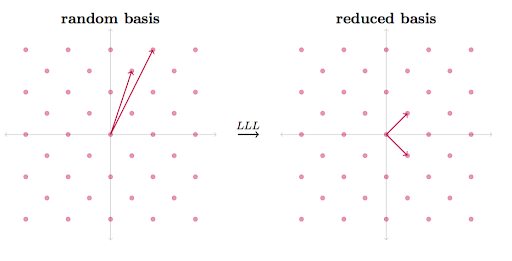
\includegraphics[width=0.8\linewidth,height=6cm]{pictures/basis_reduction.png}
\caption{Σχηματική απεικόνιση της αναγωγής βάσης κατά LLL, όπου διακρίνεται τόσο η ορθογωνιότητα των διανυσμάτων, όσο και η συρρίκνωσή τους.}
\label{fig:LLL}       
\end{figure}

Ιδιαίτερη σημασία για τη χρήση του αλγορίθμου LLL έχει το παρακάτω θεώρημα, βάση του οποίου ο αλγόριθμος επιτυγχάνει πολυωνυμική σύγκλιση. 

\begin{theorem}: 
Για μία n-διάστατη βάση $B = \{\bm b_1, ..., \bm b_n \} $, ο αλγόριθμος LLL με $ \delta = 3/4 $ έχει πολυωνιμική πολυπλοκότητα ως προς το μήκος των διανυσμάτων της βάσης και συγκεκριμένα: $ O(n^4log_2Μ) $, όπου $ Μ = \max_i(\| \bm b_i\|^2)$.
\end{theorem}
\emph{Απόδειξη.} \cite{journals/siamcomp/NguyenS09}

\section{Πρόβλημα Εύρεσης Μικρότερου Διανύσματος}
\label{chapSVP}

Στην παρούσα πτυχιακή εργασία όπως έχουμε ήδη αναφέρει, ασχολούμαστε με την επίλυση του προβλήματος μικρότερου διανύσματος SVP. Προηγουμένως, αναφερθήκαμε σε αλγορίθμους που προσεγγίζουν το πρόβλημα ως αναγωγή της δοθείσας βάσης (lattice reduction). 

Συγκεκριμένα αυτοί οι αλγόριθμοι, επιχειρούν διαδοχικούς μετασχηματισμούς στη βάση του πλέγματος, προκειμένου να καταλήξουν με μικρότερα και όσο το δυνατόν ορθογώνια διανύσματα, δίνοντας έτσι απάντηση και στο $SVP_\gamma $. Μολονότι για συνήθεις παραμέτρους απαιτούν πολυωνυμικό χρόνο, ο παράγοντας προσέγγισης $ \gamma $ που πετυχαίνουν είναι ασυμπτωτικά εκθετικός. Στην υλοποίησή μας, επιλέξαμε να χρησιμοποιήσουμε μία διαφορετική αλγοριθμική τεχνική, αυτή της απαρίθμησης. Στη συνέχεια παρουσιάζουμε τη συγκεκριμένη οικογένεια αλγορίθμων. 

\subsection{Αλγόριθμος απαρίθμησης \lt KFP}

Δοθείσας μίας βάσης $ B = \{\bm b_1, ..., \bm b_n \} $ και ενός άνω ορίου $ R $ για το ελάχιστο μήκος διανύσματος $ λ_1(L) $, αναζητούμε όλα τα διανύσματα $\bm v \in L - \{{\bf 0}\} $ που ικανοποιούν τη συνθήκη $ \| \bm v \| \leq R $.

Για το σκοπό αυτό, ο αλγόριθμος δημιουργεί ένα δέντρο απαρίθμησης (enumeration tree) που αποτελείται από όλα τα διανύσματα των πλεγμάτων προβολής $ \pi_n(L), \pi_{n-1}(L), ..., \pi_1(L) $, μέτρου το πολύ $ R $. Πιο συγκεκριμένα, το δέντρο απαρίθμησης έχει βάθος $ n $ και σε κάθε επίπεδο $ k $ βρίσκονται όλα τα διανύσματα του πλέγματος $ \pi_{n+1-k}(L) $, υπό τον περιορισμό πάντοτε ότι η νόρμα τους δεν ξεπερνά το όριο $ R $. Στη ρίζα του δέντρου βρίσκεται το μηδενικό διάνυσμα $ \bm 0 = \pi_{n+1}(L) $. Η διάταξη αυτή των διαδοχικών προβολών, μας εξασφαλίζει ότι όλοι οι πρόγονοι ενός κόμβου, έχουν το πολύ το ίδιο μήκος με τον κόμβο που έπεται. Δηλαδή:

$$ \| \pi_n( \bm v) \|^2 \leq \| \pi_{n-1}( \bm v) \|^2 \leq ... \leq \| \pi_1(\bm v) \|^2 = \| \bm v \|^2 \leq R^2 $$

Επίσης ένα διάνυσμα $ \bm v $ μπορεί να γραφτεί ως $ \bm v = u_1 \bm b_1 + \cdots + u_n \bm b_n $, όπου 

$$ \bm b_i = \bm b_i^* + \sum_{j=1}^{i-1} μ_{i,j} \bm b_j^* $$

Δηλαδή:

$$ \bm v = \sum_{j=1}^n(u_j + \sum_{i=j+1}^n μ_{i,j} u_i) \bm b_j^*, $$

οπότε και για τις νόρμες των προβολών έχουμε:

\begin{equation}
    \| \pi_{n+1-k}(\bm v) \|^2 = \sum_{j=n+1-k}^n  \bigg( u_j + \sum_{i=j+1}^n μ_{i,j} u_i  \bigg) ^2 \| \bm b_j^* \|^2, 1 \leq k \leq n. 
\end{equation}

Προκύπτει λοιπόν ένα σύνολο $ n $ ανισοτήτων. Αν ξεκινήσουμε από το $ \pi_n( \bm v)$, το οποίο ορίζεται μόνο από το διάνυσμα βάσης $\bm b_n $, μπορούμε να αποφανθούμε για το διάστημα στο οποίο επιτρέπεται να λάβει τιμές, ο αντίστοιχος συντελεστής του διανύσματος αυτού. Έχοντας βρει (απαριθμήσει) τις ακέραιες πιθανές τιμές για τον πρώτο συντελεστή, μπορούμε να προχωρήσουμε στη δεύτερη ανισότητα και να εξασφαλίσουμε τις τιμές και για τον δεύτερο.

Η διαδικασία επαναλαμβάνεται διαδοχικά για όλες τις ανισότητες, οπότε και προκύπτει το δέντρο απαρίθμησης με όλους τους πιθανούς συντελεστές για κάθε $\bm b_i $, ανά επίπεδο. Ειδικά για τον πρώτο συντελεστή περιορίζουμε την αναζήτηση μόνο σε θετικές τιμές, καθώς διαφορετικά θα οδηγούμασταν σε ένα συμμετρικό δέντρο, λόγο του ότι, αν $ \bm x \in L $ και $ - \bm x \in L $ .

Σημειώνουμε, ότι το πλήθος των κόμβων του δέντρου, εξαρτάται και από την ποιότητα της βάσης, για αυτό συνηθέστερα πριν την εφαρμογή του αλγορίθμου απαρίθμησης προηγείται κάποια αναγωγή βάσης, όπως η LLL.  

Η διάσχιση τώρα του δέντρου απαρίθμησης γίνεται κατά βάθος, με χρήση του αλγορίθμου DFS, ώστε να έχουμε μειωμένες απαιτήσεις μνήμης. Αν ο αλγόριθμος καταλήξει σε κάποιο φύλλο του δέντρου, επιστρέφει το σχηματιζόμενο διάνυσμα, υπό την προϋπόθεσή ότι το μήκος του δεν ξεπερνά το όριο $R$. Η εκτέλεση του αλγορίθμου μπορεί να είναι αποτυχημένη, αν δεν βρεθεί κάποιο άλλο διάνυσμα πέρα από το μηδενικό. Στη συνέχεια παραθέτουμε σε μορφή ψευτοκώδικα τον αλγόριθμο που μόλις περιγράψαμε.   


\begin{algorithm}[h] \label{KFP}
\SetAlgoLined

{\bf Είσοδος:} Μία βάση $ B = \{\bm b_1, ..., \bm b_n \} $ του $ \mathbb{R}^n $, η οποία ορίζει το πλέγμα $ L(B) $ και ένα θετικό αριθμό R.  \\
{\bf Έξοδος:} Τα διανύσματα $ \bm x \in L $ με $ \| \bm x \| \leq R $.

\hfill

$ B^*, μ = LLL(B) $ \# Calculate a reduced base with an algorithm such as LLL \\
$ \bm x = (x_i) \gets \bm 0_n, c = (c_i) \gets \bm 0_n, l = (l_i) \gets \bm 0_n $ \\
$ sumli \gets 0, S = \emptyset, i \gets 1 $

\While{$ i \leq n $} {
    $ c_i \gets - \sum_{j=i+1}^n x_j μ_{ji}$  \\
    $ l_i \gets B_i(x_i - c_i)^2 $ \\
    $ sumli \gets \sum_{j=1}^n l_j $ \\
    \eIf{$ sumli \leq R^2 $}{
         \eIf{$ i = 1 $}{
            $ S \gets S \cup \{ \sum_{j=1}^n x_j b_j \} $ \\
            $ x_1 \gets x_1 + 1 $ \\
        }
        {
            $ i = i - 1 $ \\
            $ x_i \gets - \sum_{j=i+1}^n μ_{j,i} x_j - \sqrt{\frac{R^2 - \sum_{j=i+1}^n I_j}{B_i}} $ \\ \# left end of interval $ I_i$
        }
    }
    {
        $ i = i + 1 $ \\
        $ x_i \gets x_i + 1 $ \\
    }
    
} % end of while
return $ S $

\caption{KFP Algorithm}
\end{algorithm}

Όσο αφορά την πολυπλοκότητα του αλγορίθμου KFP, αυτή είναι πολυωνυμική ως προς το πλήθος $ Ν $ των κόμβων του δέντρου απαρίθμησης. Αποδεικνύεται \cite{journals/corr/abs-0705-0965} ότι ένα άνω όριο για το πλήθος είναι αυτό $ Ν \leq n^{n/(2e)+o(n)}$ και ακόμα ότι υπάρχει πολυώνυμο $ p(x,y) \in \mathbb{R}[x,y] $, ώστε για κάθε πλέγμα τάξης $n$, διάστασης $m$ και με συντελεστές βάσης που φράσονται από το $ B $, η πολυπλοκότητα του αλγορίθμου να είναι: 

$$ p(log_2(B), m) n^{n/(2e)+o(n)} $$  

\subsection{Βελτιστοποιήσεις του αλγορίθμου απαρίθμησης }

Σε αυτήν παράγραφο αναφέρουμε κάποιες σημαντικές βελτιστοποιήσεις που έχουν προταθεί για τον αλγόριθμο KFP. Αρχικά οι \lt Schnorr-Euchner πρότειναν ο συντελεστής $ x_i $ αντί να λαμβάνει διαδοχικά τιμές από την αρχή του διαστήματος $ I_i $ , να εκκινεί από την ποσότητα: $ \lceil \sum_{j=i+1}^n μ_{j,i} x_j \rfloor $, που βρίσκεται περίπου στη μέση του διαστήματος $ I_i $ και κατόπιν να αυξάνεται είτε να μειώνεται κατά 1. Η συγκεκριμένη παραλλαγή ονομάζεται και αλγόριθμος απαρίθμησης των Schnorr-Euchner.

Μία άλλη παραλλαγή του βασικού αλγορίθμου, εισάγει κάποιους όρους φθοράς $ a_i \in (0,1) $ με τους οποίους αναπροσαρμόζουμε το όριο αποδοχής ως $ R_i = a_iR $ για κάθε βάθος $ i $. Η παραλλαγή αυτή ονομάζεται και απαρίθμηση με κλάδεμα. Στόχος είναι να περιορίσουμε το υπολογιστικό κόστος, μειώνοντας το χώρο αναζήτησης διανυσμάτων. Ωστόσο, είναι πιθανό ο αλγόριθμός μας να μην επιστρέψει κάποια λύση, παρόλο που μπορεί να υπάρχει διάνυσμα με μήκος μικρότερου του $ R $.  

%\subsection{\lt Pruning}

% \newpage



\section{Υλοποίηση}
\label{chapImplementation}

Στο παρόν κεφάλαιο βρίσκεται ο πυρήνας της εργασίας μας. Αρχικά γίνεται η παρουσίαση των εργαλείων, στα οποία βασίστηκε η υλοποίησή μας, ενώ στη συνέχεια παρατίθενται οι μέθοδοι κατανομής και παραλληλοποίησης, του αλγορίθμου απαρίθμησης Schnorr και Euchner. Τέλος, εκτίθεται το εργαλείο που αναπτύχθηκε στα πλαίσια της εργασίας, με σκοπό την προσομοίωση της κατανεμημένης λειτουργίας υλοποίησης. 

\subsection{Τεχνολογίες και μέθοδοι υλοποίησης}

\subsubsection{Γενικά χαρακτηριστικά}

Η ανάπτυξη της εργασίας καθορίστηκε από δύο παράγοντες. Ο πρώτος ήταν η ταχύτητα εκτέλεσης, ενώ ο δεύτερος, η ευκολία ανάπτυξης και διανομής της υλοποίησης. Οι δύο αυτοί παράγοντες υπαγόρευσαν τη χρήση τριών διαφορετικών γλωσσών προγραμματισμού, αλλά και την εκμετάλλευση δύο framework, του OpenMP για την παραλληλοποίηση των διεργασιών και του ZeroMQ για την κατανομή τους σε κόμβους του δικτύου.  

Επιπλέον, χρησιμοποιήθηκαν τα εργαλεία AsyncIO και FPLLL, που αποτελούν προγραμματιστικές βιβλιοθήκες και αφορούν αντιστοίχως, την εφαρμογή ασύγχρονων μεθόδων προγραμματισμού και την επίλυση δύσκολων μαθηματικών προβλημάτων σε πλέγματα. Η ενορχήστρωση αυτή, οδήγησε στη δημιουργία ενός λογισμικού, που υπολογίζει προσεγγιστικά τη λύση του Shortest Vector Problem, ενώ παράλληλα μπορεί να διαμοιρασθεί εύκολα μέσω της πλατφόρμας λογισμικού ανοιχτού κώδικα Docker. 


\subsubsection{Κριτήρια επιλογής γλωσσών προγραμματισμού}

Οι γλώσσες προγραμματισμού που χρησιμοποιήθηκαν, απαρτίζουν ένα δυνατό προγραμματιστικό πακέτο, το οποίο μπορεί να αποφέρει υψηλές ταχύτητες εκτέλεσης, ευκολία ανάπτυξης λογισμικού, ευανάγνωστο και συνοπτικό κώδικα. Αυτός ο συνδυασμός, έχει ως πυρήνα του, τη νέα, υβριδική γλώσσα προγραμματισμού Cython, στην οποία και υλοποιήσαμε τους βασικούς αλγορίθμους της λύσης μας. 

Η Cython \cite{cython}\cite{bCython} μπορεί και συνδυάζει την ευκολία στην ανάπτυξη προγραμμάτων της Python, μειώνοντας δραματικά τα υπολογιστικά έξοδα κατά το χρόνο εκτέλεσης, προσφέροντας απόδοση εκτέλεσης αντίστοιχης αυτής των C-Compiled προγραμμάτων. Παράλληλα, διάφορες επεκτάσεις του λογισμικού, σημεία που απαιτούσαν προγραμματιστικές τεχνικές χαμηλότερου επιπέδου αλλά και δαπανηροί υπολογιστικοί αλγόριθμοι, υλοποιήθηκαν σε C++  και στη συνέχεια διοχετεύθηκαν στον κώδικα της Cython.  

Ενώ ο πυρήνας είναι κράμα Cython και C++, το κέλυφος έχει συνταχθεί σε Python. H Python προσφέρει την ευκολία της ταχύρρυθμης ανάπτυξης κώδικα, καθώς λόγω της ευρείας υιοθέτησής της, συνοδεύεται από μία πληθώρα  πακέτων και εργαλείων ( πχ ZeroMQ, AsyncIO, FPYLLL). Ταυτόχρονα είναι απόλυτα επεκτάσιμη και φορητή, με κύριο γνώρισμά της τον συνοπτικό και ευανάγνωστο κώδικα που παράγει . Επίσης, η Python\city{HighPython} βρίσκεται προεγκατεστημένη στα περισσότερα εμπορικά και μη λειτουργικά συστήματα, κάτι που διευκολύνει τον διαμοιρασμό των αναπτυσσόμενων προγραμμάτων. Οι παραπάνω αναφορές επαληθεύουν τις προσδοκίες για το προγραμματιστικό πακέτο των αναγκών μας, καλύπτοντας όλες τις απαιτήσεις που φέρει το παραγόμενο λογισμικό. 


\subsubsection{Το \lt framework OpenMP}

Σύμφωνα με το νόμο του Moore "ο αριθμός των τρανζίστορ σ' ένα ολοκληρωμένο κύκλωμα διπλασιάζεται κάθε δύο χρόνια" κάτι που οδηγεί σε μεγαλύτερη συχνότητα, συνεπώς υψηλότερο κόστος ενέργειας. Τη λύση στο πρόβλημα αυτό δίνει η παραλληλοποίηση, όπου αντί για έναν επεξεργαστή υψηλής συχνότητας μπορούμε να έχουμε πολλούς χαμηλότερης. Ο τρόπος αυτός δεν προσφέρει υψηλότερη ταχύτητα υπολογισμών, αλλά κερδίζουμε τη δυνατότητα εκτέλεσης πολλών υπολογισμών ταυτόχρονα. Γι' αυτό και σήμερα κυκλοφορούν αποκλειστικά και μόνο πολυπύρηνοι επεξεργαστές.  

Τα σύγχρονα λειτουργικά συστήματα κατανέμουν την πληθώρα των διεργασιών τους σε διαφορετικούς πυρήνες, ενώ η ίδια διαδικασία μπορεί να υλοποιηθεί και στις εφαρμογές. Οι κατηγορίες  του παράλληλου προγραμματισμού είναι τρεις. Εμείς στην παρούσα εργασία θα αξιοποιήσουμε τις δύο εκ αυτών, την Message-Passing Programming  και την Shared-Memory Programming. Η τελευταία θεωρείται ως το απλούστερο μοντέλο παράλληλου προγραμματισμού και εφαρμόζεται στο framework OpenMP, το οποίο και αξιοποιούμε. 

  

To OpenMP (Open Multiprocessing) \cite{openmp08} είναι ένα Application Programming Interface ( API ) που υποστηρίζεται από τη C/C++, τη Fortran, πλέον και τη Cython, διαμέσω της C++  και διατίθεται για τα περισσότερα σύγχρονα λειτουργικά συστήματα όπως Linux, MacOS, Windows. Στην ανάπτυξη του λογισμικού της παρούσας εργασίας χρησιμοποιήθηκε το OpenMP σε δύο φάσεις, συμβάλλοντας στην παράλληλη εκτέλεση των ιδιαίτερα "βαριών" σημείων, που έφεραν υψηλό υπολογιστικό κόστος. Η πρώτη φάση αφορά την κλασική χρήση του, αποτελούμενη από εντολές, συναρτήσεις και μεταβλητές σε μέρος του προγράμματος που έχει συνταχθεί σε C++ ενώ η δεύτερη ποικίλλει και αφορά την παραλληλοποίηση τμημάτων της Cython.  

Η Cython παρουσιάζει γενικότερα ιδιαιτερότητες ως γλώσσα προγραμματισμού, καθώς προσπαθεί να συνδυάσει με τον καλύτερο δυνατό τρόπο τις δυνατότητες δύο πολύ ισχυρών γλωσσών. Η γλώσσα αυτή δεν είναι thread-safe - τα νήματα του επεξεργαστή δουλεύουν αποκλειστικά στο δικό τους κομμάτι μνήμης- καθώς το Global Interpreter Lock (GIL) -λειτουργία που βοηθάει στη διαχείριση μνήμης της Python και της Cython- είναι ενεργοποιημένη ώστε να εμποδίζει πολλαπλά νήματα των πυρήνων του επεξεργαστή (threads) να εκτελέσουν μεταγλωττισμένα τμήματα κώδικα της Python (python's bytecodes). Εξαιτίας αυτού λοιπόν και αφού απενεργοποιηθεί το GIL, υλοποιεί την παραλληλοποίηση μέσω μίας μεθόδου της, που ονομάζεται prange, η οποία στο παρασκήνιο εκμεταλλεύεται το OpenMP για το διαμοιρασμό μνήμης και την πολυεπεξεργασία. 

\subsubsection{Το \lt framework ZeroMQ}


Ένας από τους σημαντικότερους αν όχι ο σημαντικότερος λόγος χρήσης το ψηφιακών συστημάτων σήμερα είναι η επικοινωνία, ενώ ο τρόπος ορθής διεξαγωγής της μεταξύ συστημάτων απασχολεί το κοινό τους, καθ΄ όλη τη διάρκεια της ύπαρξής τους. Το ZeroMQ \cite{zeroMQ}\cite{zeroMQHitjens} είναι μια προγραμματιστική βιβλιοθήκη που διευκολύνει την ασύγχρονη ανταλλαγή μηνυμάτων, μεταξύ κατανεμημένων ή συγχρονισμένων εφαρμογών, χωρίς την ανάγκη ύπαρξης προγράμματος διαμεσολάβησης, που να μεταφράζει τα μηνύματα από το επίσημο πρωτόκολλο ανταλλαγής του αποστολέα, στο αντίστοιχο του παραλήπτη.  

Το framework αυτό αποτελεί μία υψηλού επιπέδου προσέγγιση, εμπεριέχοντας εύκολη και γρήγορη ανταλλαγή μηνυμάτων βασισμένη σε sockets. Χρησιμοποιώντας ένα επίπεδο αφαίρεσης, επιτρέπει στον χρήστη να εφαρμόσει υψηλού επιπέδου τεχνικές, με ταχύτητες που εμφανίζονται μόνο σε χαμηλού επιπέδου υλοποιήσεις. Επιπλέον, εφαρμόζει ασύγχρονη υλοποίηση των sockets βάση της οποίας η φυσική σύνδεση, η εγκατάσταση, η επανασύνδεση, η αποτελεσματική μεταφορά των δεδομένων μεταξύ των κόμβων του δικτύου, βρίσκονται υπό ευθύνη του ZeroMQ και  δεν απασχολούν τον χρήστη. Ακόμη υλοποιεί τους τρεις βασικούς τύπους επικοινωνίας request-reply, publish-subscribe και pipeline με μεγάλη ευκολία ως προς την εφαρμογή, τροποποίηση και ανάπτυξη τους. Παρέχει έτσι δυνατότητες δημιουργίας σύνθετων μοντέλων επικοινωνίας χωρίς ιδιαίτερο κόπο. Τα προαναφερθέντα είναι αναγκαία και ικανά για τη σύσταση του δικού μας μοντέλου επικοινωνίας, μεταξύ των κόμβων του δικτύου, το οποίο συστήνουμε στην πορεία της εργασίας. 

\subsubsection{Το εργαλείο \lt AsyncIO}

Με την έλευση των πολυπύρηνων επεξεργαστών, οι έννοιες του παράλληλου προγραμματισμού και του προγραμματισμού ταυτοχρονισμού που προϋπήρχε, άρχισαν να συγχέονται από πολλούς. Ο προγραμματισμός με ταυτοχρονισμό \cite{ConcurentDist} σε αντίθεση με τον παράλληλο προγραμματισμό μπορεί και απευθύνεται τόσο σε μονοπύρηνα όσο και πολυπύρηνα συστήματα, καθώς η ιδέα που τον διέπει είναι η "αξιοποίηση του συστήματος, δια της εκτέλεσης μιας διεργασίας όταν αυτό είναι αδρανές, περιμένοντας την απόκριση μιας άλλης προηγηθείσας διεργασίας".  

Η προγραμματιστική βιβλιοθήκη της Python, AsyncIO \cite{asyncIO}\cite{uAsync}, υλοποιεί αυτή την ιδέα, δίνοντας μία εναλλακτική στη χρήση παράλληλου προγραμματισμού καθώς μπορεί και επιτελεί διεργασίες ταυτόχρονα, αποφεύγοντας τις δυσκολίες που περιέχει η παραλληλοποίηση. Ακόμη, δίνει τη λύση σε συστήματα εξυπηρέτησης (servers), προσφέροντας τη δυνατότητα διαχείρισης πολλών χιλιάδων ταυτόχρονων αιτημάτων από ένα και μόνο σύστημα. Η βιβλιοθήκη αυτή, αποτελεί πλέον μέλος των νέων εκδόσεων της Python, και η εφαρμογή της δε θα μπορούσε να λείπει από το framework ZeroMQ, όπως και απ' την ανάπτυξη της παρούσας εργασίας. 

\subsubsection{Το εργαλείο \lt FPLLL}

Η κοινότητα προγραμματιστών ανοιχτού κώδικα έχει προσφέρει πληθώρα εργαλείων, διευκολύνοντας έτσι το έργο, τόσο της επιστήμης όσο και της βιομηχανίας. Το FPLLL ανήκει σ' αυτή τη συλλογή εργαλείων ανοιχτού κώδικα, παρέχοντας υλοποιήσεις εφαρμοσμένων αλγορίθμων στην κρυπτογραφία με πλέγματα (lattice-based cryptography). Αλγόριθμοι παραγωγής πλεγμάτων, διάφορες εφαρμοσμένες πράξεις σ΄ αυτά, όπως η αναγωγή LLL, HKZ, BKZ, καθώς και η επίλυση του SVP και του CVP με περιορισμένες δυνατότητες, μπορούν να αξιοποιηθούν διαμέσου του εργαλείου. Το FPLL διατίθεται μέσω της πλατφόρμας GitHub ενώ παράλληλα έχει αναπτυχθεί ένας Python wrapper αυτού (FPYLLLL) τον οποίο και αξιοποιούμε. 


\subsection{Κατανεμημένη προσέγγιση υλοποίησης}

\subsubsection{ Γενικά Χαρακτηριστικά}

Ένα σύνολο από αυτόνομα υπολογιστικά συστήματα (κόμβοι) που συνδέονται μεταξύ τους και παρουσιάζονται στους χρήστες τους ως κάτι το ενιαίο και συνεκτικό, αποτελούν ένα κατανεμημένο σύστημα \cite{DistributedSystems}. Σ' αυτήν την ιδέα θεμελιώνεται η υλοποίηση της εργασίας, καθώς διασφαλίζεται η διαμοίραση πόρων και επικοινωνίας, πετυχαίνοντας την καλύτερη σχέση μεταξύ απόδοσης και κόστους. Επιπλέον θεωρείται μία αξιόπιστη και ασφαλής λύση, με κύριο χαρακτηριστικό τις δυνατότητες επεκτασιμότητας του συστήματος. 

Γι' αυτό το σκοπό, αναπτύχθηκε ειδικό λογισμικό για κατανεμημένα συστήματα (Middleware) με τη βοήθεια του framework ZeroMQ και του εργαλείου AsyncIO. Το λογισμικό αυτό, παρέχει υψηλού βαθμού διαφάνεια (transpareny), συγχρονισμό μεταξύ των υπολογιστικών συστημάτων (concurrency), ανεξαρτησία από το λειτουργικό σύστημα που διαθέτει ο κάθε κόμβος (openness), διαχείριση των πόρων του εκάστοτε συστήματος (resource sharing), ενώ είναι κλιμακούμενο (scalability) και χαρακτηρίζεται από ανεκτικότητα σε σφάλματα (fault tolerance). 
 

 \begin{figure}[!htbp]
\centering
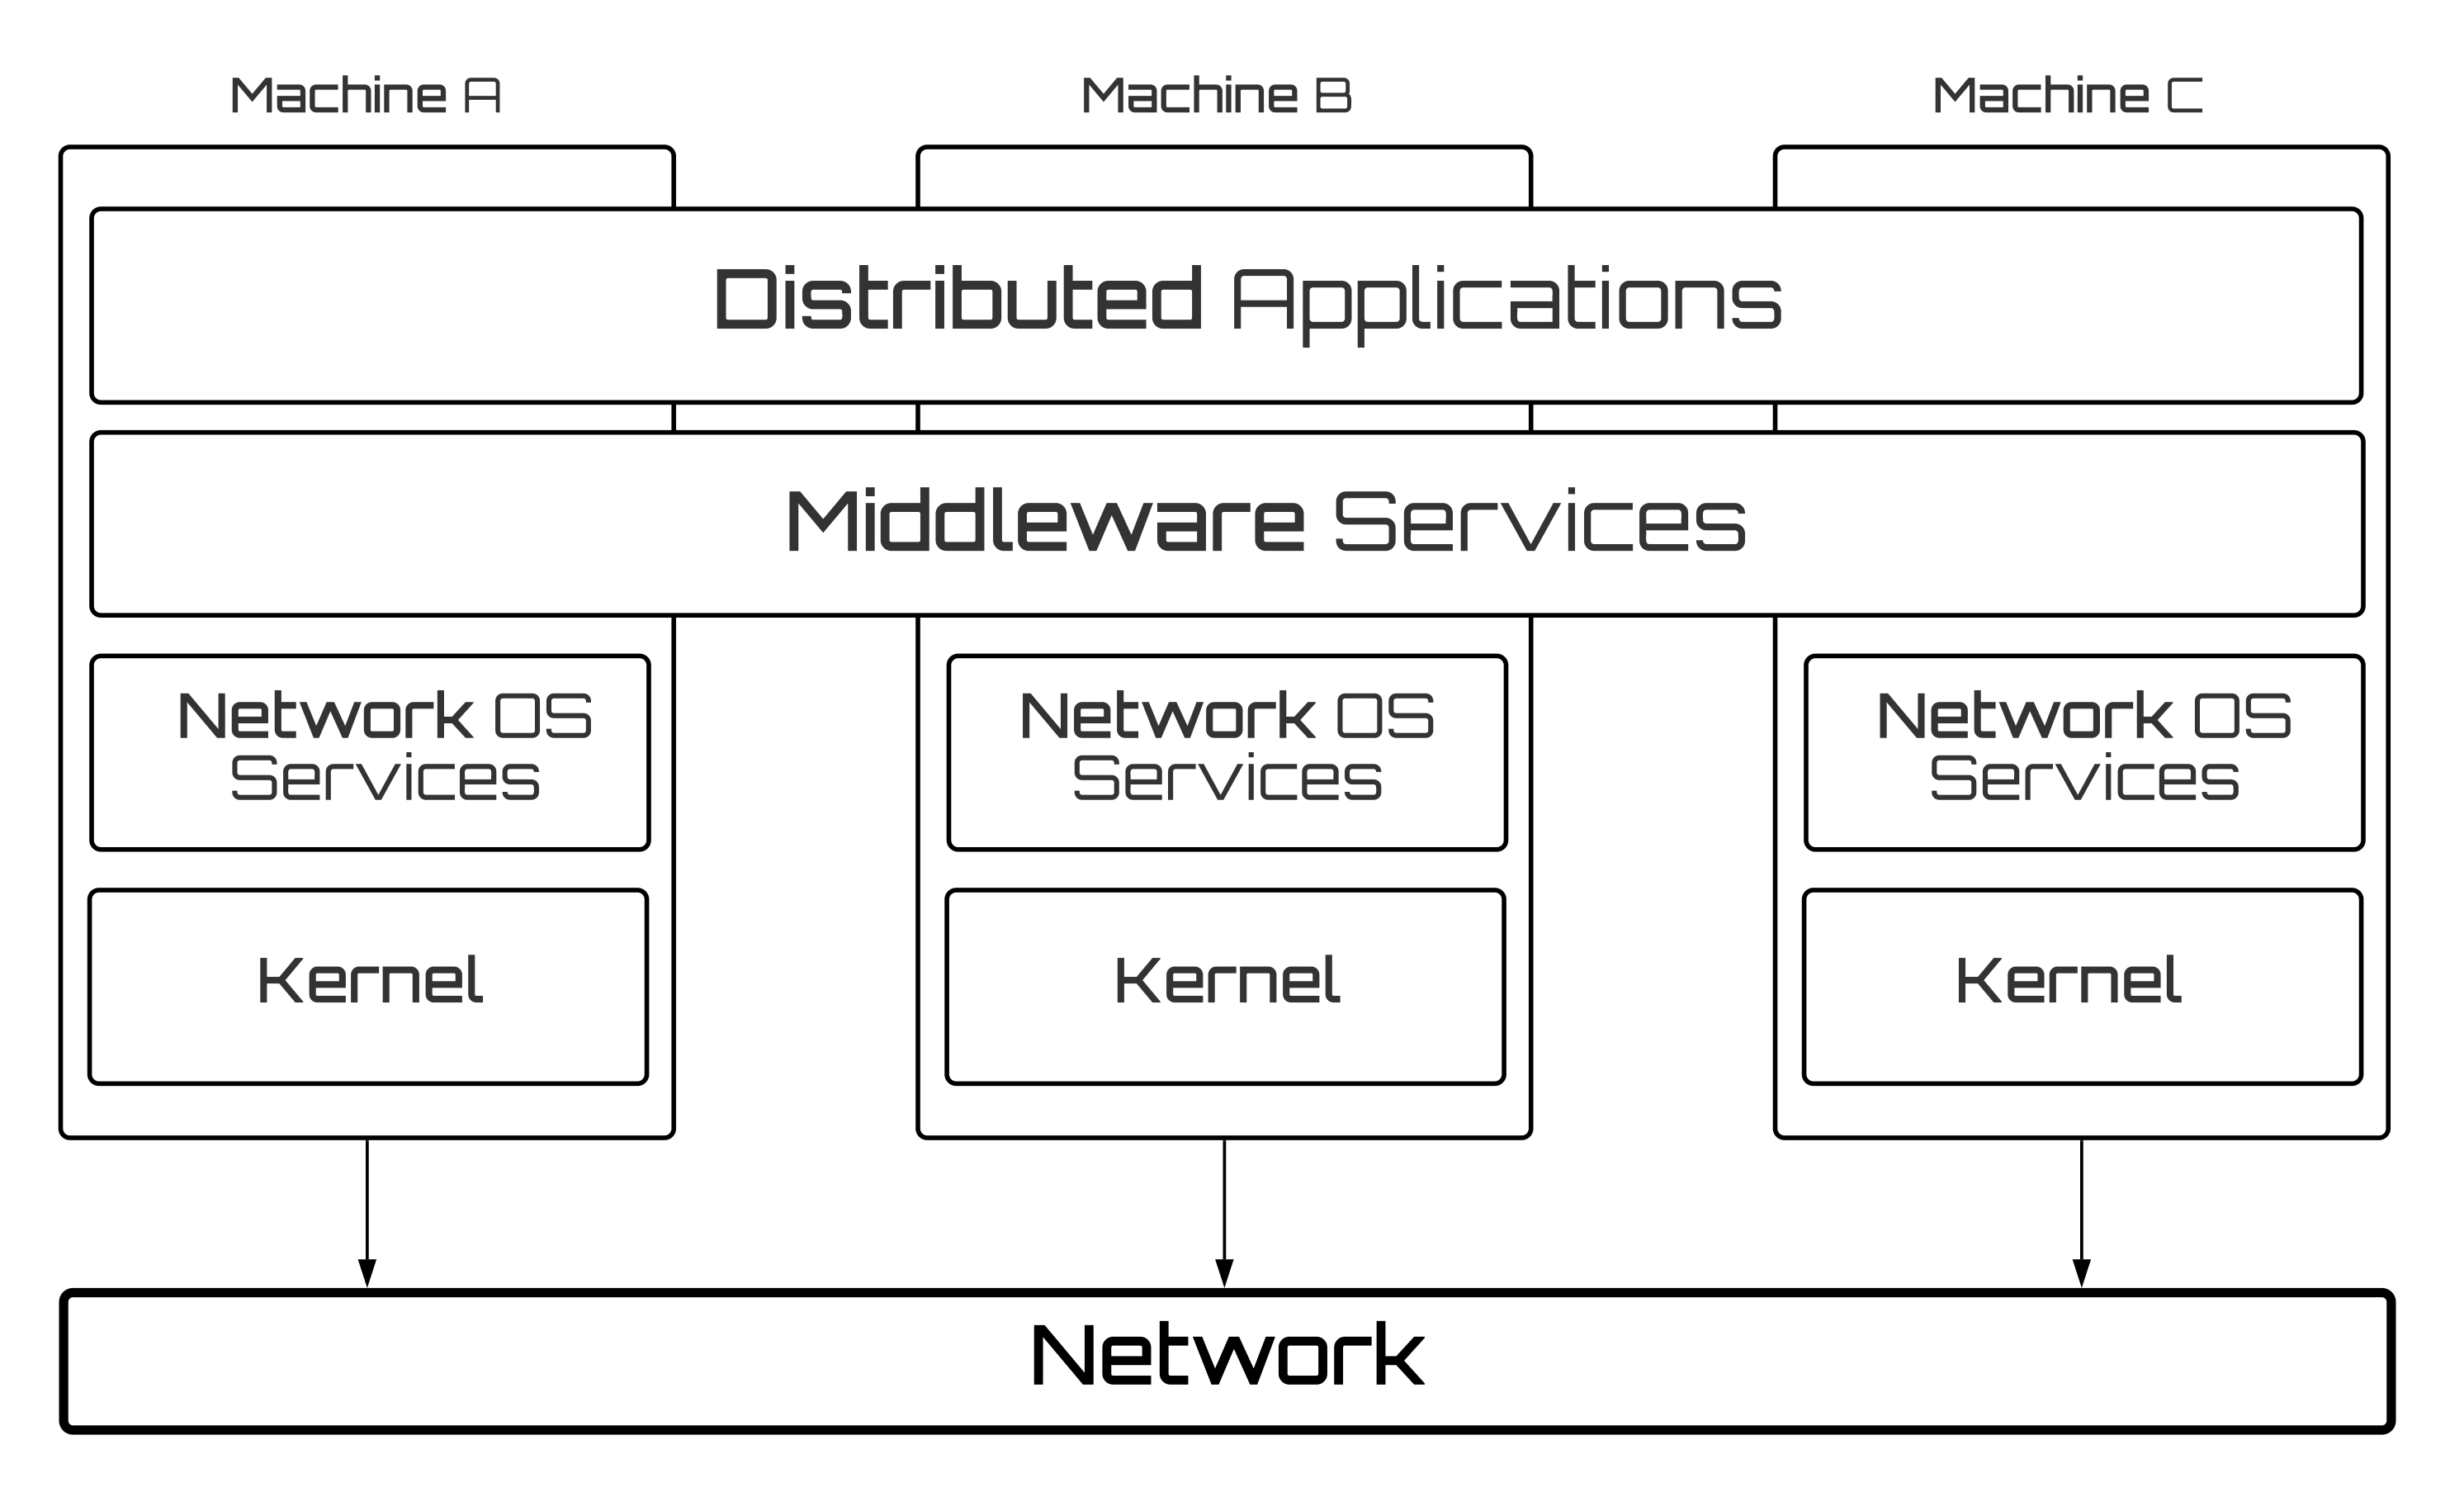
\includegraphics[width=0.8\linewidth,height=6cm]{pictures/midleware_repr_new_new.png}
\caption{Γενική δομή ενός κατανεμημένου συστήματος ως middleware.}
\label{fig:middleware}       
\end{figure}
 
 Τα χαρακτηριστικά που προσδοκήσαμε να αποδώσουμε στο middleware που παράχθηκε, βασίστηκαν στο μοντέλο κατανεμημένων συστημάτων Processor \mbox{Pool} Model (PPM) και την αρχιτεκτονική δικτύου, διαίρει και βασίλευε (Divide and Conquer - Parallel Pipeline). Το πρότυπο PPM απέφερε κατανεμημένη επεξεργασία υψηλής απόδοσης, η οποία θεωρείται απόγονος της κατηγορίας του παράλληλου προγραμματισμού Message-Passing Programming, που προαναφέρθηκε. 

 Το σύνολο των κόμβων διατηρεί σταθερή τη λειτουργία του, ανεξάρτητα με την τοποθεσία και τον τρόπο που διεξάγεται η αλληλεπίδραση μεταξύ του χρήστη και του συστήματος, δηλώνοντας τη συνοχή του. Η αρχιτεκτονική του δικτύου πετυχαίνει μέσω της παραλληλίας που τη διέπει, υψηλές επιδόσεις σε αλγορίθμους, ενώ παρέχεται ως βασικό πρότυπο σχεδίασης δικτύου, μέσω του ZeroMQ. Η ανάλυση των χαρακτηριστικών θα ακολουθήσει παρακάτω. 
 
 \subsection{Αρχιτεκτονική δικτύου}
 
Οι ανάγκες παραλληλίας, ταχύτητας και κλιμάκωσης είναι αυτές που καθόρισαν το μοντέλο που επιλέχθηκε ως βάση για την ανάπτυξη του δικτύου. Όπως και προαναφέρθηκε το μοντέλο που στηριχθήκαμε είναι το Divide and Conquer, το οποίο ονομάζει το ZeroMQ ως Parallel Pipeline. Το πρότυπο αυτό της παραλληλίας δίνει τη δυνατότητα συμμετοχής ακαθόριστου πλήθους συστημάτων-εργατών (worker), οι οποίοι δέχονται εντολές από ένα κεντρικό υπολογιστικό σύστημα (ventilator) και αποστέλλουν τα αποτελέσματα στο τελικό σύστημα συγκέντρωσης αποτελεσμάτων (sink).  
  
\begin{wrapfigure}{r}{0.5\textwidth}
    \centering
    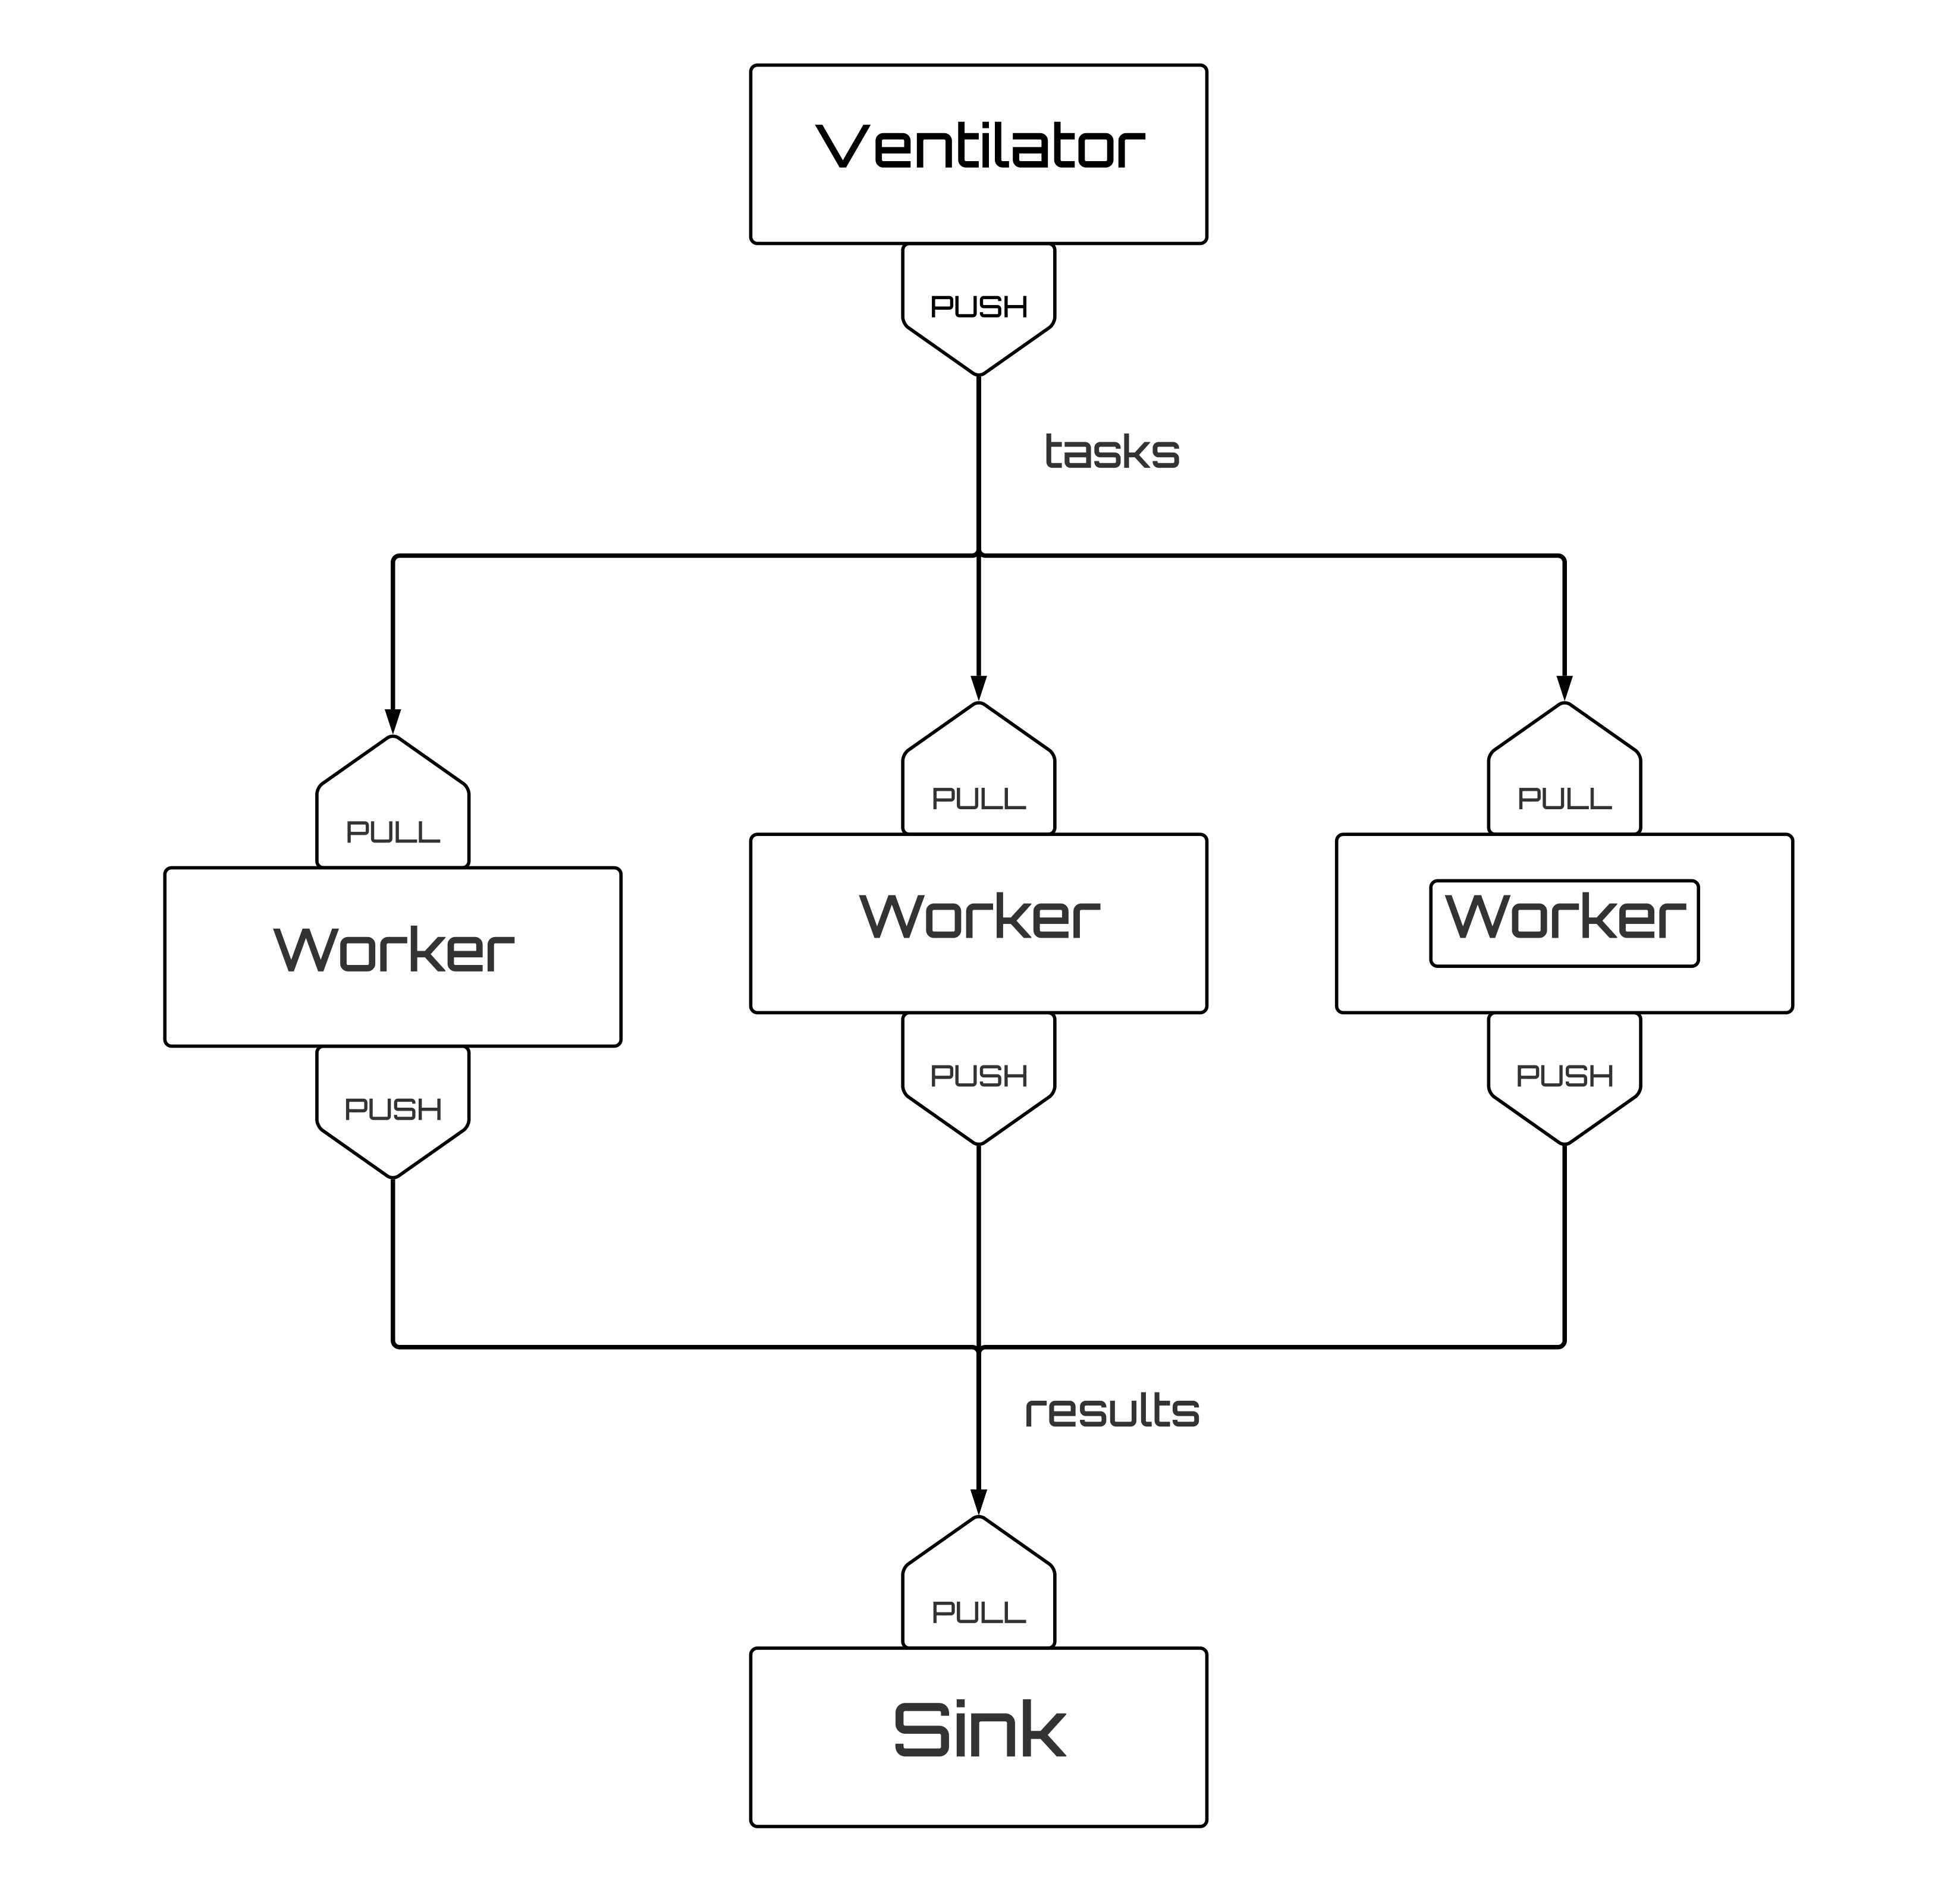
\includegraphics[width=0.4\textwidth, height=7cm]{pictures/ParallelPipeline_new.png}
    \caption{Καθορισμός Parallel Pipeline. } % σύμφωνα με το ZeroMQ.
\end{wrapfigure}  
  
  
% \begin{figure}[!htbp]
% \centering
% 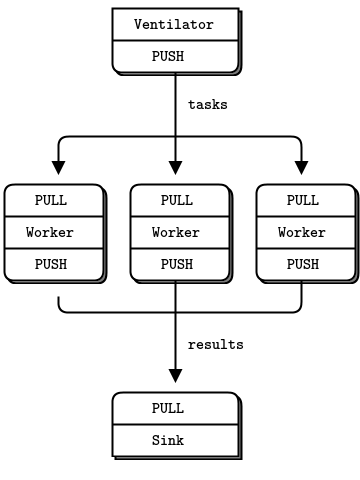
\includegraphics[width=0.8\linewidth,height=12cm]{pictures/ParallelPipeline.png}
% \caption{Καθορισμός Parallel Pipeline σύμφωνα με το ZeroMQ.}
% \label{fig:pipeline}       
% \end{figure}

Το μοντέλο που αναπτύχθηκε στα πλαίσια της εργασίας, αποτελεί μία παραλλαγή του παραπάνω έχοντας μίας βασική προσθήκη και αρκετές εσωτερικές τροποποιήσεις, έτσι ώστε να επιτευχθούν υψηλότερες επιδόσεις. Όπως παρατηρείται και στην απεικόνιση του κατανεμημένου συστήματος παρακάτω, η προσθήκη βρίσκεται στο κεντρικό σύστημα (server) με την προσάρτηση του κόμβου υποβοήθησης (secretary). Ο κόμβος-secretary αφού αλληλοεπιδράσει με τον κόμβο-server, εφαρμόζοντας το πρότυπο αίτημα-απάντηση (request-reply), μεταδίδει με χρήση του προτύπου μετάδοσης-εγγραφής (publish-subscribe) δεδομένα στους κόμβους-worker. Κάθε νέος κόμβος-worker που εισάγεται στο κατανεμημένο σύστημα, ώστε να ενισχύσει με την επεξεργαστική του ισχύ το σύστημα, λαμβάνει πρώτα μηνύματα εγγραφής (subscribe) από τον κόμβο-secretary. 

Οι κόμβοι-worker αφού λάβουν πληροφορίες (info) από τον βοηθητικό κόμβο (secretary), επικοινωνούν με το κόμβο-server εφαρμόζοντας το μοντέλο parallel pipeline. Το σύστημα συγκέντρωσης αποτελεσμάτων είναι ο κόμβος-δοχείο (pot). Οι κόμβοι-worker εκτελούν κάθε διεργασία (task) που λαμβάνουν από τον κόμβο-server, και αποστέλλουν τα αποτελέσματα (result) στο σύστημα συγκέντρωσης αποτελεσμάτων (pot), η διαδικασία αυτή επαναλαμβάνεται έως ότου ο κόμβος κόμβος-server διακόψει τη λειτουργία του. O τελικός κόμβος-pot αφού έχει λάβει στην αρχή τις απαραίτητες πληροφορίες, δέχεται επαναλαμβανόμενα τα αποτελέσματα των κόμβων-worker και στο τέλος ανακοινώνει τη λύση του προβλήματος. Το συνολικό σύστημα που προκύπτει θεωρείται συνεκτικό πληρώντας τις αρχές που διέπουν ένα κατανεμημένο σύστημα. 

\begin{figure}[!htbp]
\centering
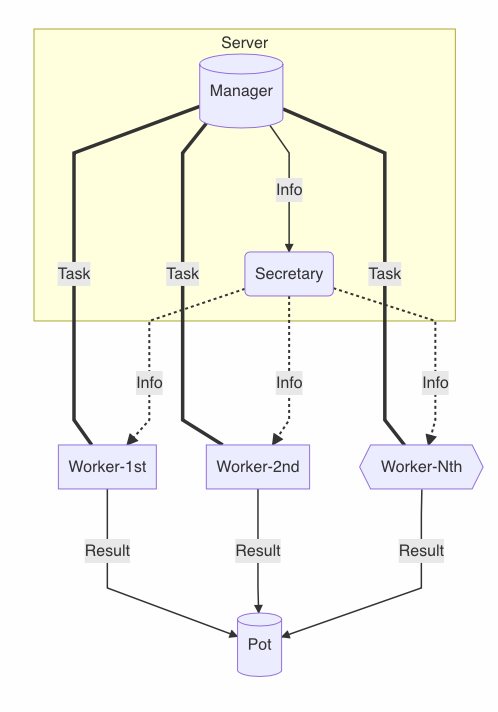
\includegraphics[width=0.8\linewidth,height=12cm]{pictures/PipelineWorkflow.png}
\caption{Διάγραμμα απεικόνισης της γενικής δομής του κατανεμημένου δικτύου.}
\label{fig:workflow}       
\end{figure}

\subsubsection{Δυνατότητες κόμβων}

Το κατανεμημένο σύστημα που παρουσιάζεται, επιτρέπει την απόκρυψη ενδεχόμενων λαθών από τον τελικό χρήστη. Αυτό πρακτικά σημαίνει ότι, τα προγράμματα εφαρμογών μπορούν να συνεχίζουν τις ενέργειές τους παρά την πιθανή αποτυχία κάποιου τμήματος του hardware ή του software, εφαρμόζοντας την αρχή της διαφάνειας αποτυχίας. Το ZeroMQ είναι αυτό που αναλαμβάνει τη διαχείριση μίας τέτοιας κατάστασης αποτυχίας, απομονώνοντας το πρόβλημα, ώστε να μην επηρεάσει το συνολικό σύστημα και επιχειρώντας να επανακάμψει από την κατάσταση σφάλματος, εάν αυτό καθίσταται δυνατόν. 

% Δηλαδή έστω ένας κόμβος-worker που αποτυγχάνει στη διεκπεραίωση της διεργασίας που του έχει ανατεθεί. Το γεγονός αυτό δεν μπορεί να επηρεάσει τη συνολική λειτουργία του κατανεμημένου συστήματος, ενώ παράλληλα ο κόμβος-pot αντιλαμβάνεται την αποτυχία του κόμβου-worker.
%, χωρίς να επηρεασθεί η λειτουργία του. 

Συνεχίζοντας, σύμφωνα με τη διαφάνεια διανομής, ένας χρήστης του κατανεμημένου συστήματος δεν είναι σε θέση να γνωρίζει που πραγματοποιήθηκε ένας υπολογισμός. Επίσης, μία εφαρμογή θα πρέπει να είναι αδιάφορη για το που ακριβώς βρίσκονται αποθηκευμένα τα δεδομένα, ενώ δεν της είναι γνωστό εάν αυτά έχουν αντιγραφεί ή όχι. Η διαφάνεια διανομής εφαρμόζεται και στο εν λόγω σύστημα, καθώς το αρχικό πρόβλημα διασπάται σε υποπροβλήματα μέσω του server. Αυτά διανέμονται στους κόμβους-workers οι οποίοι με τη σειρά τους, δίνουν τα αποτελέσματα τους στο κόμβο-pot. Τέλος, κάποιος κόμβος-worker δεν δύναται να γνωρίζει εάν είναι αυτός που έχει βρει τη λύση του προβλήματος, καθώς αγνοεί ακόμα και το ποιοι άλλοι κόμβοι συμμετέχουν στο σύστημα, πόσο μάλλον το ποια προβλήματα επιλύουν εκείνοι.  \\

%, ούτε μπορεί να γνωρίζει εάν ένας άλλος κόμβος αποτελεί μέλος-worker του συστήματος, πόσο μάλλον για το ποιο υποπρόβλημα επιλύει αυτός. \\ 

\textbf{Η σημασία του κόμβου-secretary} \\

Η προσθήκη ενός επιπλέον κόμβου-secretary προσδίδει περισσότερες δυνατότητες στο κατανεμημένο σύστημα. Αρχικά επιτρέπει την είσοδο νέων κόμβων στο σύστημα σε ακαθόριστο χρόνο, υλοποιώντας το πρότυπο επικοινωνίας publish-subscribe. Κατά αυτόν τον τρόπο αποφορτίζεται ο κόμβος-server από τα αιτήματα νέων worker, ο οποίος μπορεί τώρα αδιάκοπα να επιτελεί τη λειτουργία του. 

Επιπλέον, ο όγκος του κάθε μηνύματος, που αποστέλλει ο κόμβος-server στους κόμβους-worker καθορίζεται πλέον μόνο από τη φύση του προβλήματος, χωρίς να επαναλαμβάνονται γενικές πληροφορίες, παρά μόνο εντολές για τη διεργασία που καλείται να εκτελεσθεί. Οι γενικές πληροφορίες που καθορίζουν το πρόβλημα και είναι αναγκαίες στους νέους κόμβους-worker, μεταδίδονται μόνο μέσω του secretary. Έπειτα, ο κάθε κόμβος-worker τις αποθηκεύει τοπικά, και τις χρησιμοποιεί σε κάθε νέα διεργασία που λαμβάνει από τον κόμβο-server. Το γεγονός αυτό οδηγεί σε δραματικά μικρότερο μέγεθος μηνυμάτων, άρα μικρότερη διάρκεια κωδικοποίησης/αποκωδικοποίησης τους, λιγότερα σφάλματα μετάδοσης και συντομότερη αποστολή τους. Συνεπώς ταχύτερη επικοινωνία μεταξύ server και worker. 

Σε συνδυασμό λοιπόν, με τους αλγορίθμους που αναπτύχθηκαν για τη διάσπαση του προβλήματος σε επιμέρους διεργασίες, η προσθήκη του κόμβου-secretary καθιστά το σύστημα επεκτάσιμο (sclabale). Έτσι, προσφέρεται η δυνατότητα στις εφαρμογές, να επεκτείνουν την κλίμακα τους, χωρίς να υπάρχει αλλαγή στη δομή και στους αλγορίθμους των εφαρμογών.  

% Η αρχή διαφάνειας της κλιμάκωσης του κατανεμημένου συστήματος εφαρμόζεται διαμέσου αυτών.

% Επιπλέον, η παρουσία του κόμβου-secretary μειώνει δραματικά το latency. Αυτό συμβαίνει καθώς δεν υπάρχει κάποιος διαχωρισμός νέων και παλαιών worker, ώστε να απαιτείται η εφαρμογή διαφορετικών μεθόδων που θα αποτελούσαν αιτία αύξησης του συνολικού overhead και καθυστέρησης κατά της διαδικασία δρομολόγησης. Η λειτουργία του κόμβου-server παραμένει σταθερή και επαναλαμβανόμενη καθ' όλη τη διάρκεια λειτουργίας του. 

% χρόνος που απαιτείται για τη μετάδοση ενός κενού μηνύματος μεταξύ συσχετιζόμενων κόμβων.

% Ο κόμβος-secretary αποφορτίζει τον κόμβο-server με ποικίλους τρόπους. Ο όγκος του κάθε μηνύματος που αποστέλλει ο κόμβος-server στους κόμβους-worker καθορίζεται μόνο από τη φύση του προβλήματος χωρίς να επαναλαμβάνονται γενικές πληροφορίες, παρά μόνο εντολές για τη διεργασία που καλείται ο κάθε κόμβος-worker να εκτελέσει. Οι γενικές πληροφορίες που καθορίζουν το πρόβλημα και είναι αναγκαίες στους νέους κόμβους-worker, μεταδίδονται μόνο μέσω του secretary. Έπειτα ο κάθε κόμβος-worker τις αποθηκεύει τοπικά, και τις χρησιμοποιεί σε κάθε νέα διεργασία που λαμβάνει από τον κόμβο-server, που αφορά την επίλυση ενός και μόνου συνολικού προβλήματος. Το γεγονός αυτό οδηγεί σε δραματικά μικρότερο μέγεθος μηνυμάτων, άρα μικρότερη διάρκεια κωδικοποίησης/αποκωδικοποίησης τους, λιγότερα σφάλματα μετάδοσης και συντομότερη αποστολή τους, συνεπώς ταχύτερη επικοινωνία μεταξύ server και worker. 

\subsubsection{Η λειτουργία του προσομοιωτή \lt (Simulator)}  

Στα πλαίσια της εργασίας, αναπτύχθηκε ένα λογισμικό προσομοίωσης της λειτουργίας (simulator) του παραπάνω κατανεμημένου δικτύου, για την επίλυση του προβλήματος εγγύτερου διανύσματος σε πλέγματα. Ο σκοπός που δημιουργήθηκε ήταν η απαίτηση μας να ελέγξουμε τη συμπεριφορά του κατανεμημένου συστήματος σε διάφορες καταστάσεις με διαφορετικές παραμέτρους, αλλά και η δυνατότητα που προέκυψε να εκτελέσουμε επιτυχώς το παραγόμενο λογισμικό σε κατανεμημένο σύστημα με τη χρήση ενός και μόνου πολυπύρηνου συστήματος. Οι πυρήνες του επεξεργαστή του μηχανήματος, προσομοίωσαν τη λειτουργία των διαφόρων τμημάτων του κατανεμημένου συστήματος. Η χρήση του AsyncIO επέτρεψε την προβολή της λειτουργίας όλου του συστήματος από ένα και μόνο τερματικό, εφαρμόζοντας μεθόδους ασύγχρονου \mbox{προγραμματισμού.}  

Ο προσομοιωτής υποστηρίζει Command Line Interface (CLI) σε unix-based συστήματα, όπως MacOS και Linux. Έχει τη δυνατότητα να προσομοιώσει τη λειτουργία κόμβων-worker ανάλογα με τους διαθέσιμους επεξεργαστικούς πυρήνες του συστήματος. Συνεπώς απαιτεί τουλάχιστον τετραπύρηνα συστήματα ώστε να προσομοιώσει τη λειτουργία των τεσσάρων κόμβων, 1 x server, 1 x secretary, 2 x worker και 1 x pot, που θεωρούνται τα ελάχιστα αναγκαία για την εκτέλεση ενός ολοκληρωμένου πειράματος. 

Για τις ανάγκες των πειραμάτων, σε διάφορα συστήματα αλλά και για τον εύκολο διαμοιρασμό του λογισμικού, καθώς θεωρείται ιδιαίτερα απαιτητική η παραμετροποίηση των αναγκαίων προϋποθέσεων για την εκτέλεση του, χρησιμοποιήθηκε η πλατφόρμα ανοιχτού λογισμικού Docker\cite{DockerInPractise}\cite{DockerDeepDive}. Το container docker που παράχθηκε βασίζεται στο λειτουργικό σύστημα Ubuntu, ενώ με εντολές συστήματος οργανωμένες σε αρχεία (Makefiles) γίνεται η μεταγλώττιση (compile) όλων των αρχείων πηγαίου κώδικα (source code) της εργασίας, είτε είναι σε C++, είτε σε Cython, είτε μέσω του Python-Packaging\cite{PythonPackaging} σε Python. 

Σε επίπεδο λειτουργίας, ο προσομοιωτής εκμεταλλεύεται το τοπικό εικονικό δίκτυο (localhost) που παρέχει κάθε σύστημα μέσω του λειτουργικού του συστήματος, ώστε να αποφευχθεί η φυσική διασύνδεση στο δίκτυο. Δεσμεύει ένα πλήθος από πόρτες (ports) του localhost, ανάλογο με αυτό των κόμβων που θα λειτουργήσει. Για τον λόγο αυτό προσφέρεται μέσω του simulator, λειτουργία που κλείνει όλες τις πόρτες που θα χρειαστεί η εφαρμογή για να εκτελεσθεί. Ακόμη μπορεί να καθορισθεί ο ακριβής αριθμός των κόμβων-worker που θα προσομοιωθεί, αρκεί να υποστηρίζεται από την επεξεργαστική μονάδα του συστήματος, όπως επίσης και τα νήματα (threads) που είναι διαθέσιμα προς εκμετάλλευση από τα τμήματα του αλγορίθμου, που εμπεριέχουν παράλληλη επεξεργασία. Επίσης, δίνεται η δυνατότητα στον χρήστη να παραμετροποιήσει με κάθε τρόπο το πρόβλημα που καλείται να επιλύσει το σύστημα, είτε ακόμη να εισάγει ένα πρόβλημα επιλογής του. Τέλος, υποστηρίζει δύο λειτουργίες προσέγγισης της λύσης του προβλήματος, που θα παρουσιαστούν αναλυτικά στη συνέχεια. 
 
\subsection{Παραλληλοποίηση του \lt Schnorr-Euchner Algorithm}

\subsubsection{Φιλοσοφία παραλληλοποίησης}

Ο αλγόριθμος απαρίθμησης δημιουργεί στο παρασκήνιο ένα δένδρο (\mbox{enumeration} tree) το οποίο και προσπελαύνει με τη χρήση του αλγορίθμου διάσχισης γράφων Depth-First Search (DFS), με στόχο την εύρεση του διανύσματος που ικανοποιεί τις απαιτήσεις του προβλήματος. Ο αλγόριθμος DFS όπως προμηνύει και το όνομα του, διασχίζει το δένδρο σε βάθος, δηλαδή κατά μήκος του κάθε κλαδιού, έως ότου καταλήξει σ΄ ένα κόμβο-φύλλο της δενδρικής δομής, όπου ενδεχομένως αποτελεί υποψήφια λύση του προβλήματος. Η ιδέα που στηρίχθηκε η παραλληλοποίηση του αλγορίθμου Schnorr-Euchner έγκειται στην παραλληλοποίηση της αναζήτησης στο δένδρο απαρίθμησης, δηλαδή του DFS. 
 
 %  - ακυκλικός συνδεδεμένος γράφος -

Η παραλληλοποίηση στηρίζεται στην απλή ιδέα, της διάσπασης του δένδρου απαρίθμησης σε υποδένδρα. Η αρχική δενδρική δομή διασπάται σε μικρότερες, οι οποίες με τη σειρά τους διαμοιράζονται σε κατανεμημένα ανεξάρτητα συστήματα. Σε κάθε σύστημα επαναλαμβάνεται η διαδικασία διάσπασης. Ανάλογα με τους διαθέσιμους πόρους του συστήματος διασπάται το υποδένδρο σε μικρότερα, ώστε να εκτελεσθεί ταυτόχρονα σε κάθε δένδρο η αναζήτηση του μικρότερου διανύσματος. Ο τρόπος με τον οποίο εφαρμόζεται η διάσπαση σε υποσύνολα-υποδένδρα εκμεταλλεύεται την πρόταση του αλγορίθμου KFP, για τον ορισμό των διαστημάτων $ I_k $. 
 
$$ I_k = \Bigg[- \sum_{i=n+2-k}^n μ_{i,n+1-k} u_i - \sqrt{\frac{R^2 - \sum_{j=n+2-k}^n l_j}{\| \bm b_{n+1-k}^* \|}}, 
- \sum_{i=n+2-k}^n μ_{i,n+1-k} u_i + \sqrt{\frac{R^2 - \sum_{j=n+2-k}^n l_j}{\| \bm b_{n+1-k}^* \|}} \Bigg] $$
 
Έπειτα, εφαρμόζεται ο αλγόριθμος Schnorr-Euchner, σύμφωνα με τον οποίο η αναζήτηση στα διαστήματα $I_k$ ξεκινάει από τη μέση του διαστήματος. 

\subsubsection{Δυνατότητες υλοποίησης}

Η μέθοδος με την οποία γίνεται η διάσπαση του δένδρου μπορεί να διαφέρει, γι' αυτό και στην παρούσα εργασία υλοποιήθηκαν δύο προσεγγίσεις. Η πρώτη στηρίζεται στο πλήθος των διεργασιών που θεωρείται επιθυμητό να διασπασθεί το πρόβλημα, ενώ η δεύτερη στην ιδέα της διάσπασης του προβλήματος, αφού πρώτα υπολογισθούν τα διαστήματα για κάποιο συγκεκριμένος βάθος του δένδρου απαρίθμησης. Οι δύο αυτές παραλλαγές ισοδυναμούν με τις δύο διαφορετικές λειτουργίες του Simulator που αναφέρθηκαν στην προηγούμενη ενότητα. 

Η διάσπαση του δένδρου βάσει του επιθυμητού πλήθους διεργασιών, έχει καλή εφαρμογή όταν έχουμε γνώση του ακριβή αριθμού των κόμβων-worker, καθώς τότε ο διαμοιρασμός μπορεί να είναι ακριβής. Έτσι αποφεύγεται η εμφάνιση του σύνηθες προβλήματος, κατά το οποίο απομένει να εκτελείται μία περίσσεια διεργασία ενώ τα υπόλοιπα συστήματα έχουν ολοκληρώσει την επεξεργασία τους. Κάτι τέτοιο θα μπορούσε να οδηγήσει ακόμα και σε διπλασιασμό της εκτέλεσης του συστήματος. Φυσικά υπάρχουν ποικίλες λύσεις στο πρόβλημα αυτό, όπως το dynamic-scheduling ή ο αλγόριθμος Round Robin, αλλά στη δική μας περίπτωση αυξάνουν αισθητά την πολυπλοκότητα. Συνεπώς, καταλήξαμε πως εάν γνωρίζουμε τον αριθμό των κόμβων-worker, επιλέγουμε το πλήθος των διεργασιών έτσι ώστε να είναι ακέραιο πολλαπλάσιο του πλήθους των κόμβων-worker, αυξάνοντας ενδεχομένως σε κάποιες περιπτώσεις τις απαιτήσεις μερικών διεργασιών. Πιο αναλυτικά, ενώ υπό ιδανικές συνθήκες τα υποσύνολα (υποδένδρα) που διαμοιράζονται έχουν τον ίδιο αριθμό στοιχείων, σε περιπτώσεις όπως την προαναφερθείσα διαφέρουν, ώστε να μην υπάρχει πλεόνασμα, γι' αυτό και οι απαιτήσεις των διαμοιραζόμενων διεργασιών δεν είναι ισοδύναμες.  

Η έναρξη της παράλληλης επεξεργασίας αφού προϋπολογισθούν κάποια διαστήματα $ U_n,U_{n-1},...,U_k $ όπου $ k \in \mathbf{Z} $ είναι η δεύτερη λειτουργία που υλοποιήθηκε. Σύμφωνα μ’ αυτή τη λειτουργία μπορούν να κλαδευτούν κάποια υποδένδρα τα οποία δεν θα οδηγούσαν σε κάποια λύση, γι’ αυτό και συνίσταται η επιλογή του κατάλληλου $k$ μετά από ανάλογο πειραματισμό, (σ’ αυτή τη προσέγγιση θα μπορούσαν να εφαρμοσθούν τεχνικές Machine Learning για την επιλογή του $ k $). Ο ακέραιος αριθμός $ k $ συμβολίζει το βάθος που θα προσπελαθεί στο δένδρο απαρίθμησης έως ότου διασπασθεί σε υποδένδρα. Το πλήθος των διεργασιών που προκύπτει διαφέρει ανάλογα την περίπτωση, αλλά η φιλοσοφία διαχωρισμού τους είναι η ίδια μ' αυτή που εφαρμόζεται στην προηγούμενη λειτουργία. 

\subsubsection{Ανάλυση συστήματος}

Το κατανεμημένο σύστημα παράλληλης επεξεργασίας για $ m $ το πλήθος κόμβους-workers και $ n $ αριθμό νημάτων-threads σε κάθε κόμβο-worker, μπορεί να εκτελέσει παράλληλα, $ m*n $ διεργασίες. Η λειτουργία του συστήματος αυτού, παρουσιάζεται αναλυτικά στο διάγραμμα \ref{fig:system}. 

\begin{figure}[!htbp]
\centering
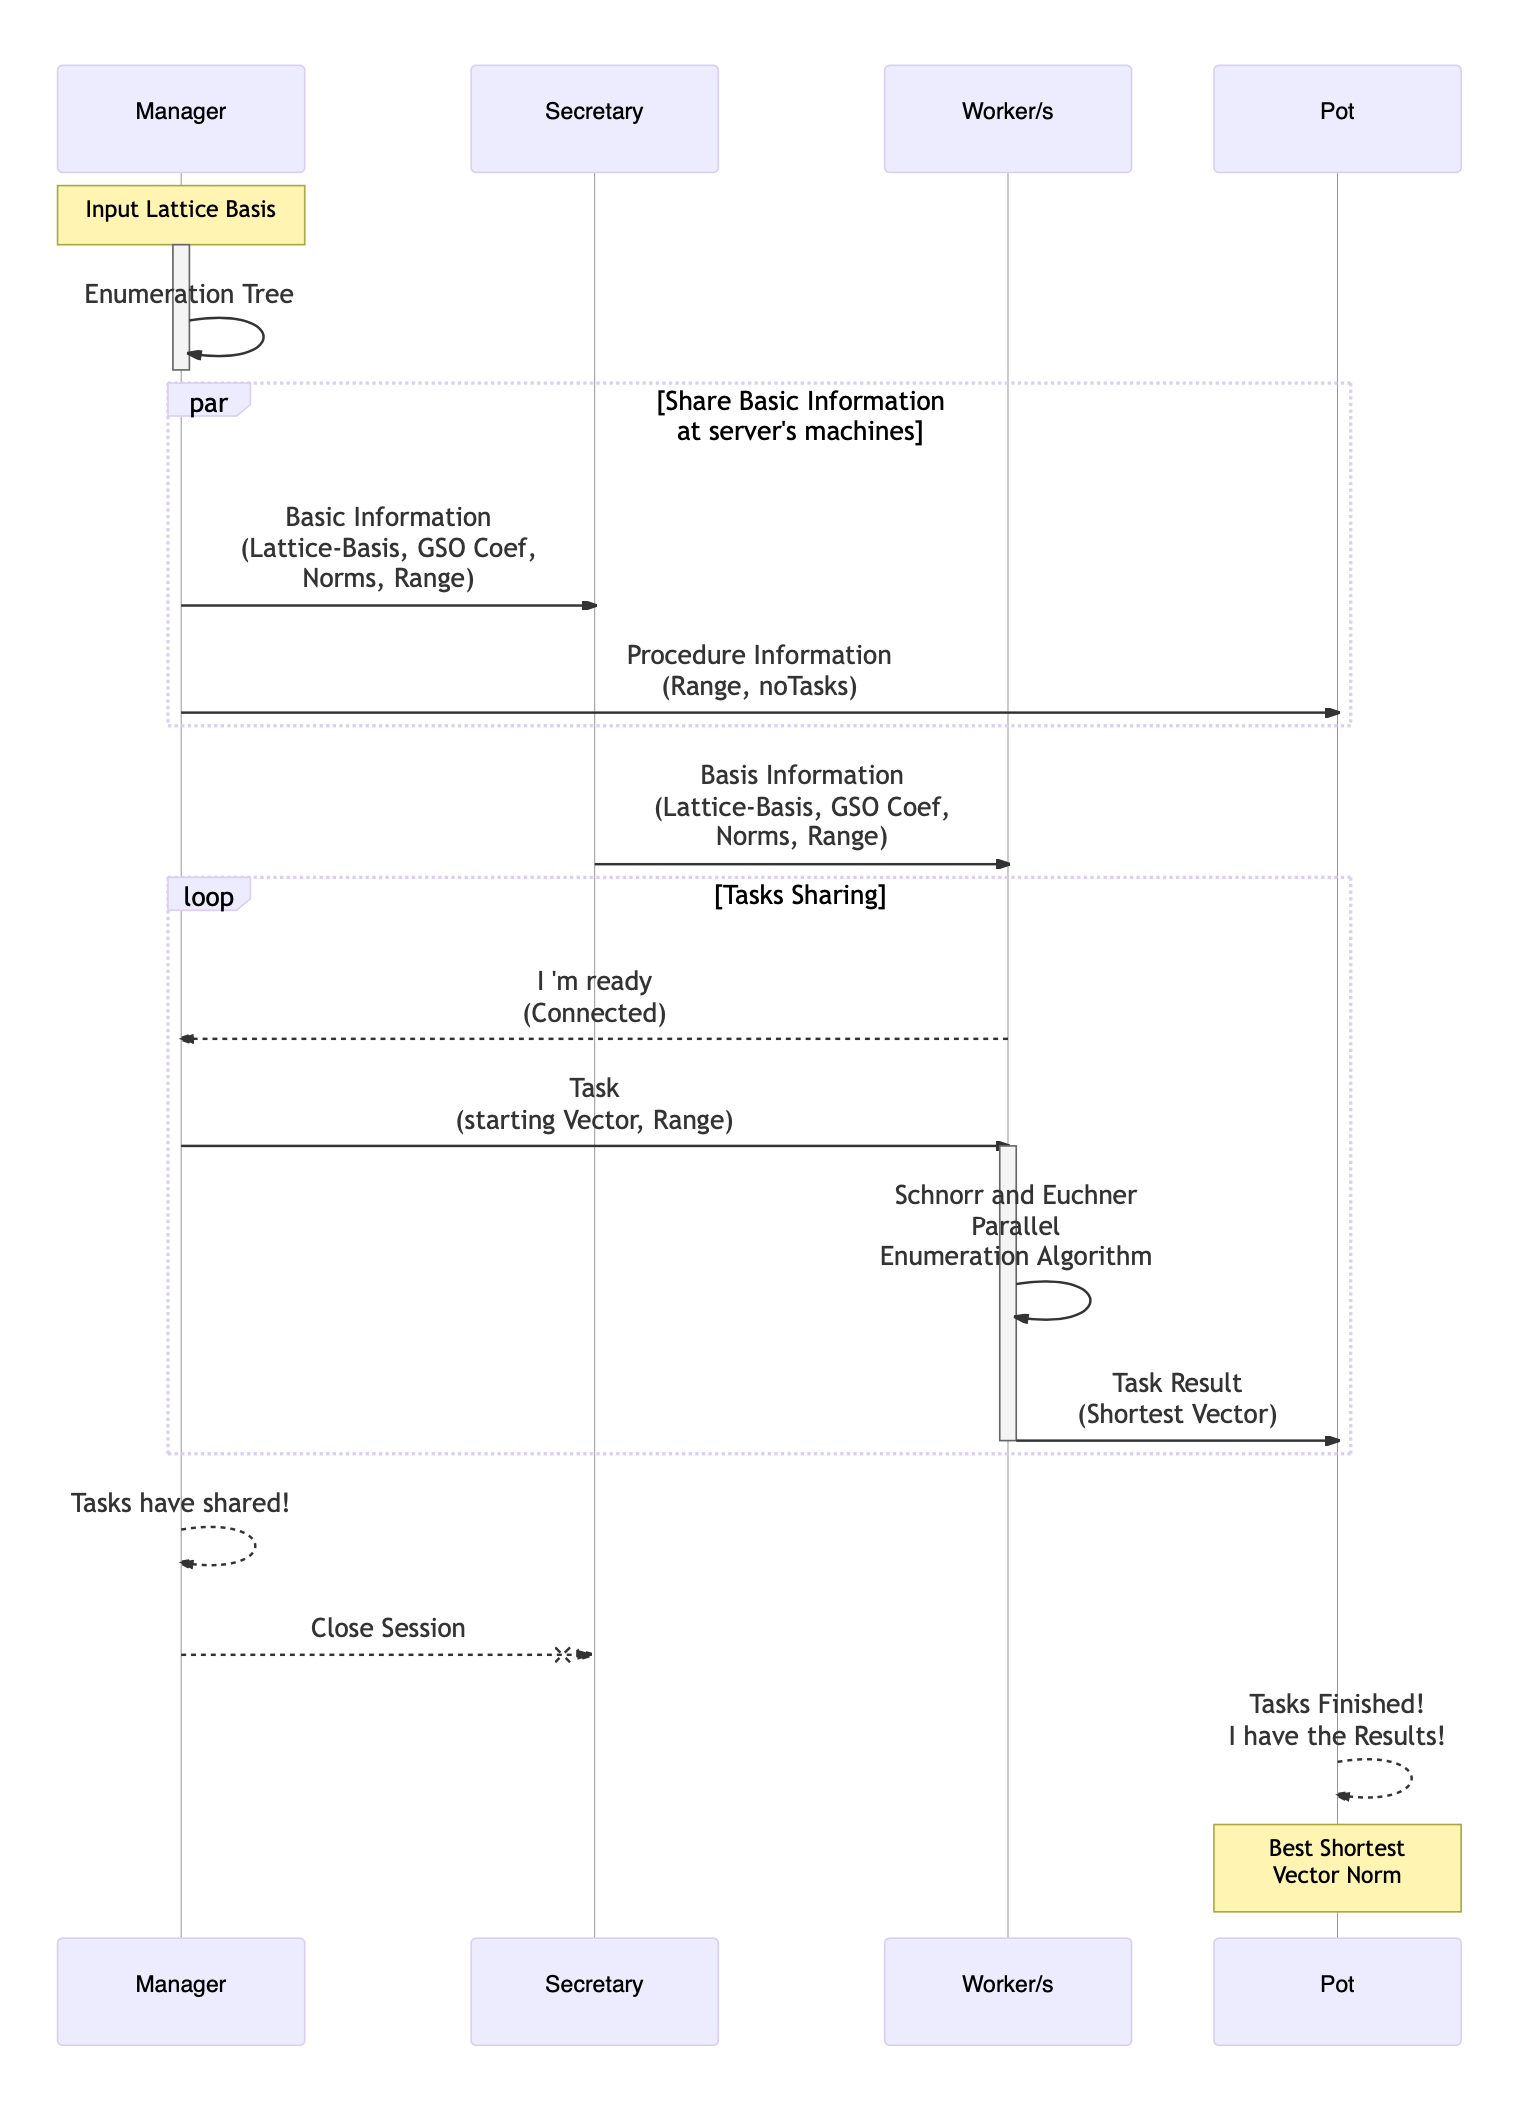
\includegraphics[width=0.8\linewidth,height=16cm]{pictures/SystemAnalysis.png}
\caption{Λειτουργία του κατανεμημένου συστήματος.}
\label{fig:system}       
\end{figure}

Έπειτα, στους αλγορίθμους που ακολουθούν παρουσιάζουμε τις μεθόδους που ακολουθήθηκαν για την επίτευξη της παραλληλίας στο συνολικό σύστημα. Η λειτουργία της διάσπασης λαμβάνει χώρα στον server node όπου δημιουργείται ένα δέντρο απαρίθμησης μέσω του αλγορίθμου \emph{4.1}, το οποίο διασπάται σε επιμέρους κλαδιά (συνδεδεμένη λίστα), που συμβολίζουν τις διεργασίες. Στη συνέχεια διαμοιράζονται σε καθέναν από τους worker nodes. Οι worker nodes αφού λάβουν τις διεργασίες, σύμφωνα με τον αλγόριθμο \emph{4.2}, τις διασπούν σε υποδιεργασίες  οι οποίες εκτελούνται παράλληλα στον επεξεργαστή του συστήματος. Κύριο μέλημα είναι καμία υποδιεργασία να μην παρεμβαίνει στο χώρο αναζήτησης κάποιας άλλης, ώστε να μην υπάρχει σπατάλη επεξεργαστικού χρόνου, αυτό επιτυγχάνεται με τον αλγόριθμο \emph{4.3}, παραλλαγή του αλγορίθμου των Schnor και Euchner\cite{journals/mp/SchnorrE94}.

\begin{algorithm}[h] \label{split}
\SetAlgoLined

{\bf Input:} $ μ, Β^*, n $  \\
{\bf Output:} Tree branches. \\

\hfill

$ B^*_i = \| b^*_i \|^2, μ = GSO(B) $ \quad \emph{\#Calculate Gram-Schmidt Orthogonalization} \\

$ tree = new \; Tree() $ \\
$ x\_vector = new \; Vector(n) $  \quad \emph{\# Fill with zeros} \\

\emph{\# Calculate $ I_k $} \\
$ upper\_bound = find\_range\_KFP(M, B^*, n, tree.height+1, x\_vector).upper\_bound $

$ tree.new\_root\_node(upper\_bound, n, x\_vector) $ \\
$ BFS = tree.iterator.begin() $ \\
$ total\_range = 1 $ \\
$ expression = distribution\_mode.expression() $ \emph{\# modes: [via\_Nodes, via\_Depth]}\\
\While{$ expression(total\_range)$} { 
    $ parent = bfs() $ \\
    $ height = parent.depth + 1 $ \\
    \If{$ n < height $}{
        \textbf{break}
    }
    $ index = n - height $ \\
    \For{$int \; i=0; \; i\leq parent.upper\_bound; \; i++$} {
        $ new\_x\_vector = parent.x\_vector $ \\
        $ nex\_x\_vector[index] = i$ \\
        $ new\_upper\_bound = find\_range\_KFP(height, new\_x\_vector).upper\_bound $ \\ 
        $ tree.new\_node(new\_upper\_bound, n, new\_x\_vector, index) $ \\
    } 
    $ total\_range += parent.upper\_bound $ \\
    $ BFS.next() $ \\

} % end of while
\textbf{return} $ tree.get\_branches() $

\caption{Sever-Node: Enumeration Tree for Distributed Operation}
\end{algorithm}





\begin{algorithm}[h] \label{split-worker}
\SetAlgoLined

{\bf Input:} $ server\_msg, no\_threads $ \\
{\bf Output:} S \\

\hfill

$ μ = server\_msg.get\_GSO\_Coefficients() $ \\
$ B^* = server\_msg.get\_B\_norms2() $ \\
$ n = server\_msg.get\_size() $ \\
$ R = server\_msg.get\_R() $ \\
$ branch = server\_msg.get\_process() $ \\


$ x\_vector = branch.x\_vector $ \\

$ index\_border = branch.index $ \qquad \qquad \emph{\#constant}\\
\If{$ index\_border == 0 $}{
    \textbf{return} $ x\_vector $
}
$ range = branch.upper\_bound + 1 $ \qquad \emph{\#[0, branch.upper\_bound]} \\ 
$ no\_tasks = range // threads $ \qquad \emph{\#integer\ division} \\
$ balance = range \% threads $ \qquad \emph{\#modulo} \\

\If{$ no\_tasks == 0 $}{
    $ no\_threads = balance $
}
$ x\_parallel = new Array(n,\ no\_threads) $ \\
\textbf{parallel}
\For{$ t=0,\ t< no\_threads,\ t++ $}{ 
$ copy(x\_parallel[t],\ x\_vector,\ n)$
}

$ S = new \ ParallelHeap() $ \\
\textbf{parallel}
\For{$ t=1,\ t< no\_threads,\ t++ $}{
$ extra\_task = (t+balance-no\_threads)*((t+balance)>=no\_threads) $ \\
$ upper\_bound = no\_tasks*t -1 + extra\_task  $ \\
$ lower\_bound = upper\_bound + 1 - no\_tasks - ((t+balance)>=no\_threads) $\\

$ S = S \cup \{ Bounded\_SchnorrEuchner(μ,\ Β^*,\ n,\ R,$ \\ $ \qquad x\_parallel[t\_id],\ index\_border,\ lower\_bound, upper\_bound)\} $
}



\textbf{return} $ S $

\caption{Worker-Node: Schnorr-Euchner Parallel Operation}
\end{algorithm}





\begin{algorithm}[h] \label{bounded}
\SetAlgoLined

{\bf Input:} $μ, Β^*, n, R, x, i_{border}, lower\_bound, upper\_bound $,  \\
{\bf Output:} S \\

\hfill

$ \bm c = (c_i) \gets \bm 0_n, l = (l_i) \gets \bm 0_n $ \\
$ Δx \gets (1, \bm 0_{n-1}), Δ^2x \gets(1,(-1)_{n-1}), suml_i \gets 0, S = \emptyset, i \gets 0, S \gets []) $ \\

\While{$ i < i_{bound} $} { 

    $ c_i \gets - \sum_{j=i+1}^{n-1} x_jμ_{ji}$ \\
    $ l_i \gets B_i(x_i - c_i)^2 $ \\
    $ sumli \gets \sum_{j=i}^{n-1}l_j $ \\
    
    \If{$ sumli \leq R^2 $ and $ i=0 $}{
        $ S \gets S \cup \{ \sum_{j=0}^{n-1} x_j b_j \} $ \\
    }
    \If{$ sumli \leq R^2 $ and $ i>0 $}{
            $ i = i - 1 $ \\
            $ c_i \gets - \sum_{j=i+1}^{n-1} μ_{j,i} x_j $ \qquad \emph{\# center of interval $ I_{n+1-i}$} \\
            $ x_i \gets \lceil c_i \rfloor $ \\
            $ Δx_i \gets 0 $ \\
            \eIf{$ c_i < x_i $}
            {$ Δ^2x_i \gets 1 $ }
            {$ Δ^2x_i \gets -1 $}
    }
    {
    \eIf{$ i==i_{border} \ OR \ ( i==i_{border}-1 \ AND \ ( x[i] < lower\_bound \ OR \ x[i] > upper\_bound ))$}{
    \textbf{break}
    }
    {
    $ i \gets i + 1 $ \\
    $ Δ^2x_i \gets - Δ^2x_i $ \\
    $ Δx_i \gets -Δx_i +Δ^2x_i $ \\
    $ x_i \gets x_i + Δx_i $ \\
    \If{$ i==i_{border}-1 \ AND \ ( x[i] < lower\_bound \ OR \ x[i] > upper\_bound )$}{
    \textbf{break}
    }
    
    }
    
    }

} % end of while
\textbf{return} $ S $

\caption{Bounded Schnorr-Euchner Enumeration Algorithm}
\end{algorithm}


\section{Επίλογος}
\label{chapClose}
\subsection{Σύνοψη και Συμπεράσματα}

Η εργασία εκπονήθηκε μετά από συστηματική μελέτη του μαθηματικού υπόβαθρου της επιστήμης των πλεγμάτων, της κρυπτογραφίας δημοσίου κλειδιού και της ανάλυσης βέλτιστων αλγορίθμων παραλληλοποίησης και ταυτοχρονισμού. Χρησιμοποιήθηκε πληθώρα προγραμματιστικών εργαλείων, ενώ αναπτύχθηκαν και νέα εργαλεία για τις ανάγκες υλοποίησης και προσομοίωσης της λειτουργίας του συστήματος. Η συγγραφή του λογισμικού σε τρεις γλώσσες προγραμματισμού κάλυψε τις υψηλές απαιτήσεις που τέθηκαν εκ των προτέρων. 

Στόχος ήταν η επίλυση του προβλήματος του εγγύτερου διανύσματος, μέσω ενός συστήματος υψηλής απόδοσης, με ανοχή στα λάθη, πλήρως επεκτάσιμο και εύκολα διαμοιραζόμενο. Τα αποτελέσματα που προέκυψαν φανερώνουν πως η παράλληλη υλοποίηση των αλγορίθμων μπορεί να φέρει μεγέθη απόδοσης, εκθετικά μεγαλύτερα σε σύγκριση με τα γραμμικά συστήματα.  Το σύστημα ολοκληρώθηκε εκπληρώνοντας κάθε προσδοκία, όντας πλήρως λειτουργικό.

\subsection{Επεκτάσεις}

Η εργασία αυτή αποτελεί τον εναρκτήριο λίθο της ανάπτυξης ενός λογισμικού με επίκεντρο την τεκμηρίωση ασφαλείας ενός κρυπτογραφικού συστήματος βασιζόμενο σε πλέγματα. Τα επόμενα βήματα ανάπτυξης θα μπορούσαν να περιέχουν, την προσθήκη αλγορίθμων επίλυσης σε CUDA, που εκτελούνται σε κάρτα γραφικών, ώστε να αξιοποιείται πλήρως κάθε σύστημα. Επίσης την εφαρμογή τεχνικών βελτιστοποίησης σε αλγορίθμους που αναπτύχθηκαν. Επιπλέον τη δημιουργία ενός συστήματος παροχής υπηρεσιών ιστού μέσω του οποίου διευκολύνεται η συμμετοχή νέων κόμβων στο κατανεμημένο σύστημα και τελος τη διεξαγωγή πειραμάτων ευρείας κλίμακας υπό πραγματικές συνθήκες.


%%%%%%%%%%%%%%%%%%%%%%%%%%%%%%%%%%%%%%%%


% Βιβλιογραφία - Αναφορές

	%\bibliography{references}
        \begin{otherlanguage*}{english}
		\bibliography{biblio}
		\end{otherlanguage*}
	\bibliographystyle{plain}
	
% Παραρτήματα
	%\appendix
% 	\chapter{Παραρτήματα}



\section{Εγκατάσταση του {\lt CUDA} για {\lt Ubuntu linux}}

Πριν φτάσουμε στην εγκατάσταση του CUDA πρέπει πρώτα να ελέγξουμε κάποια πράγματα. 

1. Ελέγχουμε αν η GPU που έχουμε υποστηρίζει CUDA. Αυτό μπορεί κάποιος να το ελέγξει από το site\lt \footnote{\label{note1}  \url{ https://www.geforce.com/hardware/technology/cuda/supported-gpus?field_gpu_type_value=All}} της NVIDIA που περιέχει τη λίστα με τις GPU που υποστηρίζουν CUDA. 


\newpage 

\section{Εκτέλεση του κώδικα}
Η σειρά εκτέλεσης της πτυχιακής με τις κατάλληλες εντολές είναι η εξής:

1. Πρώτα εκτελούμε το πρόγραμμα με όνομα {\lt ArrayProduction.c} για να παράξει έναν τυχαίο πίνακα από 0 και 1. Οι εντολές είναι
a) gcc ArrayProduction.c -o ArrayProduction (-std=c99 για cc=1.x)
b) ./ArrayProduction 10 (όπου 10 είναι το μέγεθος του πίνακα, για να δημιουργηθεί ένα πίνακας $10 \times 11$)



	\include{end_sections/glossary}	
	\nocite{*}
	
	\appendix

%%%%%%%%%%%%%%%%%%%%%%%%%%%%%%%%%%%%%%%%%%%%%%%%%%%%
%\backmatter
% Ευρετήριο Όρων
%	\printindex
%	\cleardoublepage

\end{document}
